%=== CHAPTER FIVE ===
%% Implementation and experimental evaluation.  Rewritten 2026-10-30 for the
%% 14-state mass-only interface (full-state estimator); 2026-11-05: Section
%% sec:eval:reduced adds the full-state versus reduced estimator comparison.  The frozen cohort of the previous
%% revision used a different estimator configuration and is not reused.
%% 2026-11-03: cohort results filled from final_cohort_20261030_190107
%% (analysis/summary.md, scripts/gripper/aggregate_final_cohort.py) and the
%% residual ablation from l1_ablation_20261101_020253.  Draft notes remain only
%% where no batch in the evaluated configuration exists yet.
%% 2026-11-03 (later): restructured into 5.1-5.9; experiments without results
%% moved to Section 5.8 (not run) and Chapter 6; no numbers changed.
%% 2026-11-05: added Section 5.6 (force-balance release campaign, 312 flights,
%% release_paper_20261103_210022, scripts/gripper/aggregate_release_paper.py);
%% not-run / missing-baseline / thrust-calibration text updated accordingly.
%% 2026-11-06: implementation and default statements aligned with the mainline
%% code base (MHE_NMPC, commit 5b7881e): deployed system = reduced estimator R +
%% force-balance release rule (arm D); switchable arms, the full-state estimator
%% and the comparison controllers remain in the campaign code base (ros2_ws_HJH).
%% No experimental number changed.
%% 2026-11-07: Section sec:eval:deployed added (180-flight deployed-system
%% validation, R + arm D, mainline tag deployed-r-armd-180-v1, analysis in
%% results/campaign_180_analysis/, scripts/tools/campaign_eval.py); it is the
%% primary evidence.  Cohort and 312-flight campaign kept as historical (F).

\chapter{Implementation and Experimental Evaluation}
\label{ch:evaluation}
\begin{spacing}{1.5}
\setlength{\parskip}{0.22in}

This chapter addresses the fifth research objective: evaluating the complete
interface in software-in-the-loop simulation and characterising where it fails.
The evidence comes from sources of different standing, which are kept apart
throughout (Section~\ref{sec:eval:evidence}). The primary evidence for the
deployed system --- the reduced estimator with the force-balance release rule
--- is a campaign of $180$ flights of that system under nominal release,
delayed detachment, uncommanded loss, a jammed gripper and thrust-map error
(Section~\ref{sec:eval:deployed}). The remaining sources concern the
\emph{historical} configuration in which the design was developed, with the
full-state estimator: a frozen, block-randomised cohort of $120$ flights on the
estimator's mass evidence (Sections~\ref{sec:eval:cohort}--\ref{sec:eval:results});
a second frozen campaign of $312$ flights that introduced the force-balance rule
and compared fixed and $\mathcal{L}_1$ baselines
(Section~\ref{sec:eval:campaign}); a smaller frozen batch that isolates the
residual specific force; and the paired comparison of $96$ flights on which the
reduced estimator was chosen (Section~\ref{sec:eval:reduced}). Development
flights in earlier configurations are used only to show mechanisms. The frozen
campaign of an earlier revision used a different estimator and eccentric grasps;
none of its numbers is reused here.

\section{Platform and Implementation}\label{sec:eval:platform}

The implementation is organised as ROS~2 packages around PX4
software-in-the-loop \cite{px4} and Gazebo \cite{gazebo}. The controller node
owns the reference generator, the predictive optimal control problem, the mission
sequence and the release-confirmation logic; the estimator node owns the sliding
measurement window, the physical-input reconstruction, the mass optimisation, the
presence machine and the published payload frame. The two communicate through the
single atomic frame of Section~\ref{sec:frame:interface}.

\begin{table}[ht]
\centering
\caption[Main implementation components]{Main implementation components. Rows
marked $^{\ast}$ exist only in the campaign code base; the others form the
deployed pipeline.}
\label{tab:software}
\small
\begin{tabularx}{\textwidth}{@{}l X X@{}}
\toprule
\textbf{Component} & \textbf{Role} & \textbf{Principal signals} \\
\midrule
Gazebo (Harmonic) & Rigid-body physics; detachable-joint gripper &
pose, rotor speed, attach/detach record (logging only) \\
PX4 SITL & State estimation, rate loop, control allocation &
odometry, actuator commands \\
\texttt{mhe\_node} & moving-horizon mass estimation (full-state in the campaigns, reduced deployed); presence machine &
odometry, rotor speed $\rightarrow$ payload frame \eqref{eq:frame} \\
\texttt{acados\_nmpc\_node} & Predictive control, mission sequence, confirmation &
payload frame, state $\rightarrow$ thrust and body-rate setpoint \\
\texttt{acc\_release\_detector} & Force-balance release evidence
\eqref{eq:macc}--\eqref{eq:gammaacc}, inside the controller &
rotor speed, inertial specific force $\rightarrow$ $\gamma_{\mathrm{acc}}$ \\
\texttt{payload\_estimate} & Frame schema, evidence score \eqref{eq:gamma} &
shared by the online nodes and the offline replay \\
\texttt{proximity\_gripper\_node} & Grasp contact and release actuation &
proximity, grasp enable, release command \\
\texttt{lifecycle\_trace} & Machine-readable event trace for scoring &
every state transition, with timestamps \\
\texttt{l1\_adaptive} & Residual specific-force estimator
(Section~\ref{sec:model:residual}); in the campaign code base also the
comparison adaptive controller &
odometry, rotor speed $\rightarrow$ $\hat{\bm d}$ \\
\texttt{px4\_pid\_benchmark}$^{\ast}$ & Bare-autopilot cascade baseline &
position setpoints only \\
\bottomrule
\end{tabularx}
\end{table}

Every reported payload change is produced by the detachable-joint gripper,
which adds or removes a genuine second rigid body and therefore changes mass and
inertia together. A retired run-time inertia plugin did not alter the physics
engine and contributes no result to this dissertation.

Across twenty recorded batches, reconstructed roll and pitch torques track the
intended values (median correlations $0.93$ and $0.70$; slopes $1.08$ and
$1.10$), whereas executed yaw torque is only $0.32$ of the intended value. This
three-fold yaw discrepancy is a concrete reason to drive the estimator with the
measured wrench \eqref{eq:phys}, not the command.

\subsection{Platform parameters and task}\label{sec:eval:params}

The reusable-vehicle constants are
\begin{equation}
\mB=\SI{2.0643}{\kg},\qquad
\Jb=\mathrm{diag}(0.0142,\,0.0142,\,0.0210)\ \si{\kg\meter\squared},\qquad
k_d=0.05 ,
\label{eq:platform}
\end{equation}
with rotor arm \SI{0.174}{\meter}, $k_f=\SI{8.55e-6}{\newton\second\squared}$ and
$k_m=\SI{0.016}{\meter}$. The collective-thrust box is the actuator envelope
\eqref{eq:envelope}, $[\SI{1.27}{\newton},\SI{31.35}{\newton}]$, and the torque
bounds are \SI{0.5}{\newton\meter} in roll and pitch and
\SI{0.2}{\newton\meter} in yaw. None of these grows with the estimate.

The value $\mB$ appears in the model, in the derived quantity
$\mP=(\mT-\mB)^{+}$ and in offline scoring. The payload is a
\SI{0.15}{\meter} cube of \SI{0.15}{\kg} or \SI{0.30}{\kg}, placed directly
below the grasp point so that the grasp is centred. The gripper attaches when the
parcel is within \SI{0.03}{\meter} horizontally of the attachment point and its
vertical distance lies in $[\SI{0.15}{\meter},\,\SI{0.45}{\meter}]$. The
vehicle descends to \SI{0.35}{\meter} above ground to grasp, which realises a
vertical arm of about \SI{0.27}{\meter}; both optimisers use the nominal prior
$r_z=\SI{-0.27}{\meter}$, and the realised arm varies between about
\SI{0.25}{\meter} and \SI{0.30}{\meter} from flight to flight
(Section~\ref{sec:model:whynot}). None of the payload values is supplied to the
estimator or the controller.

The task sequence is: approach under position control; hand-off to the predictive
controller and warm-up hover; alignment over the parcel; controlled descent;
grasp enable; lift from \SI{0.35}{\meter} to \SI{6.0}{\meter} in
\SI{8.4}{\second}; figure-eight carry \eqref{eq:fig8} with $r=\SI{10}{\meter}$,
$z_h=\SI{6.0}{\meter}$ and $d_z=\SI{0.8}{\meter}$; release; recovery. The
release command is issued after \SI{45}{\second} of loaded figure-eight, at the
next tip of the figure-eight ($a=3\pi/2$), so that every release occurs at the
same geometric phase. The two speeds are set by the phase rate:
$w=\SI{0.283}{\radian\per\second}$ for a peak of about
\SI{4}{\meter\per\second}, and $w=\SI{0.1415}{\radian\per\second}$ with a
\SI{9.36}{\second} speed ramp for about \SI{2}{\meter\per\second}. The scope of
the controller is stated explicitly --- it governs the grasp hover and the
post-event adaptation phase, and the approach controller is not part of any
claim. Batches run headless.

\subsection{Real-time performance}\label{sec:eval:timing}

On one desktop core shared with the simulator and the autopilot, the 13-state
controller ($N=20$, \SI{20}{\hertz}) solves in \SI{1.3}{\milli\second} at the
median and \SI{2.2}{\milli\second} at the 99th percentile over $n=1009$ solves:
\SI{2.6}{\percent} and \SI{4.4}{\percent} of its \SI{50}{\milli\second} period.
The controller's problem dimensions are unchanged by the estimator
configuration.

The full-state estimator ($N=20$, \SI{10}{\hertz}) logs its solve time as a mean
and a maximum over consecutive \SI{2}{\second} windows, not per solve. Over the
$120$ cohort flights, with the first two windows of each flight discarded
($n=5800$ windows), the window mean had a median of \SI{2.8}{\milli\second}, a
90th percentile of \SI{5.4}{\milli\second} and a 99th percentile of
\SI{14.3}{\milli\second}; the largest single solve recorded in any window was
\SI{77.3}{\milli\second}. Against the \SI{100}{\milli\second} period the
estimator never overran in the cohort, but the worst case used about three
quarters of it, and because only window aggregates were recorded, the
per-solve percentiles are not available. The reduced estimator logs every solve;
its timing is reported with the deployed-system validation
(Section~\ref{sec:eval:deployed}) and the comparison of
Section~\ref{sec:eval:reduced}.

The deadline is met in simulation. We nevertheless make \emph{no} claim about
headroom on an onboard computer; that requires measurement on the target
hardware.

\section{Evaluated Configuration}\label{sec:eval:config}

Throughout this dissertation, \emph{evaluated configuration} means the
full-state (14-state) mass-only MHE of Section~\ref{sec:model:mhe} at
\SI{10}{\hertz} ($N=20$), driven by odometry and the rotor-speed wrench, with
stage weights that were uniform in effect (Section~\ref{sec:frame:beta}), the
$0.95\,\mB$ lower bound,
lagged inertia \eqref{eq:Afrozen}, $r_z=\SI{-0.27}{\meter}$, window-balance
seeding and, in the cohort, the earlier product form of the evidence score
\eqref{eq:gamma} (see \emph{Historical scoring} below). It feeds the 13-state
NMPC at \SI{20}{\hertz}. The cohort additionally
sets five non-default choices explicitly:
\begin{enumerate}
\item the residual specific force $\hat{\bm d}$ of
Section~\ref{sec:model:residual} ($a=10$, $\omega_c=\SI{0.5}{\radian\per\second}$);
\item the attach-time inertia floor held until the release command
(Section~\ref{sec:frame:bootstrap});
\item alignment relative to the parcel before grasp, to \SI{0.012}{\meter}
with at most \SI{4}{\second} of waiting (Section~\ref{sec:eval:alignment});
\item a smoothed initial yaw reference at the start of the figure-eight;
\item the shortened arm described above.
\end{enumerate}
Offset compensation is off and every grasp is centred. Inner-loop scaling and
lifecycle thresholds remain at their documented defaults; switches belonging to
the unused moment/offset formulation are inactive. Appendix~A gives the complete
resolved configuration. All $120$ flight records were checked and contain the
14-state selection, lagged inertia, residual, inertia-floor hold, relative
alignment, yaw smoothing and stated $r_z$ prior.

\paragraph{Deployed system.} The deployed system differs from the evaluated
configuration in two places: its release rule is the force-balance rule, arm~D
of Section~\ref{sec:eval:campaign}, and its estimator is the reduced
velocity--mass estimator of Section~\ref{sec:frame:redmodel}. Everything else
--- controller, residual specific force, inertia-floor hold, alignment, yaw
smoothing, arm prior, inner-loop scaling and lifecycle thresholds --- is the
configuration above. On 5 November 2026 the deployed system was extracted from
the campaign code base into a separate mainline code base in which these
settings are fixed rather than switchable (Section~\ref{sec:eval:defaults}).

\paragraph{Deployed estimator.} After the cohort and the release campaign, the
experiment entry points were switched to the reduced velocity--mass estimator of
Section~\ref{sec:frame:redmodel}. Every flight of
Sections~\ref{sec:eval:results}--\ref{sec:eval:campaign}, of the ablations other
than Section~\ref{sec:eval:reduced}, and of the failure-mode analysis was flown
with the full-state estimator from the campaign code base; those results
describe the historical configuration, not the deployed estimator. The
exceptions are the R arm of Section~\ref{sec:eval:reduced} and the $180$ flights
of the deployed-system validation (Section~\ref{sec:eval:deployed}); the latter
were flown with the deployed system itself, from the mainline code base. The
evidence for the replacement is Section~\ref{sec:eval:reduced}. Results that depend on the estimator's model ---
the mass bias and its manoeuvre-induced collapse in particular --- should not be
transferred to the reduced estimator without that evidence.

\paragraph{Historical scoring.}
The cohort of Sections~\ref{sec:eval:cohort}--\ref{sec:eval:results} was flown
with an earlier product score, which multiplied the mass score of
\eqref{eq:gamma} by an inertia score derived from the same mass estimate. Its
results are therefore reported as results of that historical configuration.
They are not a closed-loop validation of the mass-only score \eqref{eq:gamma},
and no closed-loop rerun with the mass-only score was made: the deployed system
does not release on the mass score at all, but on the force balance of arm~D
(Section~\ref{sec:eval:campaign}). Offline replay of the cohort with the
mass-only score found no change in acceptance time in 68 of 71 score-confirmed
flights and a \SI{0.1}{\second} advance in the other three. This indicates that
the two scores would have behaved alike in these flights, but it is a replay of
recorded data, not a closed-loop result.

\subsection{The full-state estimator and the mass-evidence lifecycle}\label{sec:model:mhe}

Neither belongs to the system of Chapters~\ref{ch:model} and~\ref{ch:framework};
they are stated here because every flight of
Sections~\ref{sec:eval:results}--\ref{sec:eval:campaign} and of the failure-mode
analysis used the first, and the cohort used the second.

\paragraph{Full-state estimator F.} F integrates the complete vehicle model and
augments the composite mass into its state,
\begin{equation}
x_{\mathrm{aug}} = \bigl[\,x;\; \mT\,\bigr] \in \mathbb{R}^{14},
\qquad \dot{\mT} = 0,
\label{eq:xaug}
\end{equation}
with process noise on the thirteen physical states only. Its known parameters
are the reconstructed wrench of \eqref{eq:phys} and a geometry slot,
\begin{equation}
p_{\mathrm{MHE}} = \bigl[\, \Tphys;\; \tauphys;\; \dJ^{\mathrm{est}};\; c^{\mathrm{est}}_x;\; c^{\mathrm{est}}_y \,\bigr] \in \mathbb{R}^{7},
\label{eq:pmhe}
\end{equation}
and its stage residual is the full measurement residual
\begin{equation}
\bm e_i \;=\; \bm y_i - x_i
\;=\; \bigl[\,\bm e^p_i;\ \bm e^v_i;\ \bm e^q_i;\ \bm e^{\omega}_i\,\bigr]
\in \mathbb{R}^{13},
\label{eq:mheresid}
\end{equation}
with a component-wise quaternion difference in $\bm e^q$. F keeps the mass off
the rotational channel by removing only the direct sensitivity,
\begin{equation}
\frac{\partial \dot{\bm\omega}}{\partial \mT}\bigg|_{\text{estimator}} = 0 ,
\label{eq:nodwdm}
\end{equation}
and inserts the inertia increment as a known parameter computed from the previous
solution $\hat m^{-}$ and held constant within the window,
\begin{equation}
\dJ^{\mathrm{lag}} = \frac{\mB\,\bigl(\hat m^{-}-\mB\bigr)^{+}}{\hat m^{-}}\; r_z^2,
\qquad
\frac{\partial \dJ^{\mathrm{lag}}}{\partial \mT}\bigg|_{\text{window}} = 0,
\label{eq:Afrozen}
\end{equation}
refreshed at the \SI{10}{\hertz} window rate, with the positive part smoothed over
\SI{0.02}{\kg}; the two offsets are zero. Both indirect couplings of
Section~\ref{sec:model:rotchannel} therefore remain in F. It is solved as
\eqref{eq:mhe} with $C$ selecting the thirteen vehicle states and process noise
on all of them, at the same horizon and rate as the deployed estimator, with
\begin{equation}
W_y = \mathrm{diag}\Bigl(\sigma_p^{-2}I_3,\ \sigma_v^{-2}I_3,\ \sigma_q^{-2}I_4,\ \sigma_\omega^{-2}I_3\Bigr),
\label{eq:Wy}
\end{equation}
$\sigma_p=\SI{0.02}{\meter}$, $\sigma_v=\SI{0.05}{\meter\per\second}$,
$\sigma_q=0.01$, $\sigma_\omega=\SI{0.02}{\radian\per\second}$,
\begin{equation}
W_w = \mathrm{diag}\bigl(10^{4} I_6,\ 10^{5} I_4,\ 10^{3} I_3\bigr),
\label{eq:Ww}
\end{equation}
\begin{equation}
W_0 = \mathrm{diag}\bigl(10^{3} I_6,\ 10^{4} I_4,\ 10^{2} I_3,\ \sigma_{m,0}^{-2}\bigr),
\label{eq:W0}
\end{equation}
whose velocity and mass entries are those of \eqref{eq:Wred}, so that the
comparison of Section~\ref{sec:eval:reduced} isolates the model structure rather
than a retuning. Its mass was held in a hard box $[0.95\,\mB,\ \SI{5.0}{\kg}]$
with no health check, and after five consecutive solver failures it adopted the
window-balance seed as its estimate.

\paragraph{Mass-evidence lifecycle.} The cohort accepted a release on the
estimator's mass score $\gamma$ of \eqref{eq:gamma}, in the product form noted
under \emph{Historical scoring} in Section~\ref{sec:eval:config}, instead of
$\gamma_{\mathrm{acc}}$: the persistence test of \eqref{eq:confirm},
$\gamma\ge0.90$ held for \SI{1.0}{\second}, on healthy, fresh frames. It had two
arming policies: \emph{always-on} counted the persistence throughout loaded
flight, \emph{command-armed} only after the release command. There was no loss
watchdog, the attach-time inertia floor was ended only by the release command,
and an acceptance with no command outstanding did not reset the residual
$\hat{\bm d}$. The release arms of Section~\ref{sec:eval:arms} are built on this
lifecycle.

\section{Deployed-System Validation}\label{sec:eval:deployed}

This section is the primary evidence for the system of
Chapters~\ref{ch:model} and~\ref{ch:framework} as deployed: the reduced
velocity--mass estimator R with the force-balance release rule (arm~D), and the
controller, residual specific force, inertia floor, alignment and lifecycle
settings of Section~\ref{sec:eval:config}, run from the mainline code base
(Section~\ref{sec:eval:defaults}). A campaign of $180$ flights repeats with
that system the release, fault and thrust-map experiments that the historical
release campaign of Section~\ref{sec:eval:campaign} flew with the full-state
estimator, and adds the combination that campaign did not fly: an
under-reading thrust map with delayed detachment. It is a separate batch, from a
different code base and on different days. It is not paired with, and not pooled
with, any other result of this chapter; where its results are set beside those
of the historical campaign, the comparison is descriptive.

\subsection{Design and execution}\label{sec:eval:dep:design}

The campaign uses four conditions: c1, \SI{0.15}{\kg} at
\SI{2}{\meter\per\second}; c2, \SI{0.15}{\kg} at \SI{4}{\meter\per\second};
c3, \SI{0.30}{\kg} at \SI{4}{\meter\per\second}; and c4, \SI{0.30}{\kg} at
\SI{2}{\meter\per\second}. Trajectory, grasp and release phase are those of
Section~\ref{sec:eval:params}. It has four segments
(Table~\ref{tab:dep-design}). Within each round every cell of a segment is flown
once, in an order drawn from the segment's seed, and the whole schedule was
written before the segment's first flight.

\begin{table}[ht]
\centering
\caption[Design of the deployed-system validation]{Design of the
deployed-system validation. d0: detachment at the command; d4: detachment held
\SI{4}{\second} after the command. Gain: thrust-map gain on the estimation
side (see text).}
\label{tab:dep-design}
\small
\begin{tabularx}{\textwidth}{@{}l c >{\raggedright\arraybackslash}X c@{}}
\toprule
\textbf{Segment} & \textbf{Flights} & \textbf{Factors} & \textbf{Seed} \\
\midrule
Release & 72 & d0 / d4 $\times$ c1--c4 $\times$ 9 rounds & 20261106001 \\
Faults & 48 & uncommanded loss / jammed gripper $\times$ c1--c4 $\times$ 6 rounds & 20261106002 \\
Thrust map & 48 & gain $0.90$ / $1.10$ $\times$ c1--c4 $\times$ 6 rounds; d0 & 20261106003 \\
Thrust map, delayed & 12 & gain $0.90$ $\times$ c1, c2 (\SI{0.15}{\kg}) $\times$ 6 rounds; d4 & 20261106004 \\
\midrule
Total & 180 & & \\
\bottomrule
\end{tabularx}
\end{table}

The thrust-map gain has the meaning it had in the historical campaign
(Section~\ref{sec:eval:camp:design}): it scales the thrust reconstructed from
rotor speeds in the estimator's thrust input and in the force-balance detector
\eqref{eq:macc}. The thrust used by the residual specific force, the
thrust-to-throttle map, the actuator envelope and the plant's rotor
coefficient keep the nominal $k_f$, so the error reaches the control input only
through the mass estimate. An uncommanded loss detaches the payload at the
release phase with no command and no notification; a jammed gripper receives
the normal command and never releases.

The four segments were flown back to back, from 20:15 on 6 November to 06:33 on
7 November 2026. The flight code was frozen at tag
\texttt{deployed-r-armd-180-v1} (commit \texttt{59236f7}) of the mainline code
base. A fingerprint of the flight-stack sources and configuration, the launch and
stop scripts and the batch driver was checked before every flight and was
\texttt{186022e6c95cfa38} throughout. During the release segment a commit that
changed only the sources of this dissertation (\texttt{9881e78}) moved the
repository head, so the three later segments record that commit instead of the
tag; the unchanged fingerprint shows that the flight code was the same. The
toolchain and solver identities are listed in Appendix~\ref{app:deployed-id}.
Eligibility and reruns followed rules written into the batch driver before the
first flight: only an infrastructure failure --- stack not started, logs
missing, configuration not matching the schedule, physical attachment failed, or
no trigger before the timeout --- would have been rerun, once, with the original
flight kept in the record. Divergence, solver failure, early or missed
confirmation and \textsc{unresolved} are outcomes. All $180$ flights attached
and were eligible, and none was rerun. A six-flight smoke batch, one flight per
path, preceded the campaign to check the driver and the logs; it is not part of
the results.

Repeated flights of a cell receive no seeded random input. They differ through
the simulator's unseeded sensor noise and through the timing jitter of the
simulation step and of the multi-process stack
(Section~\ref{sec:eval:stats}). Intervals therefore describe the
repeat-to-repeat variation of this simulation stack on this machine, not a
population of real flights. No significance test is made in this section, so
no correction for multiple comparisons arises.

\subsection{Acceptance criteria}\label{sec:eval:dep:accept}

The campaign had no pre-registration of its own. Its four acceptance criteria
were inherited verbatim from the pre-specification of 5~November~2026 for the
comparison of F and R (Section~\ref{sec:eval:reduced}), namely items 1, 2, 9 and
10, the items that concern R alone, with the parts that require a comparison
with F removed. They were fixed during the run: they were written to the
campaign's analysis directory after $11$ of the $180$ flights, when only the
terminal-state lines of those $11$ flights in the campaign log had been seen and
no summary had been opened, and before the three later segments started. They
were not changed afterwards. Item~8 of the earlier specification (no runs of
non-zero solver status and no re-initialisation under a \SI{-10}{\percent}
thrust map) was not adopted, and the corresponding observations are reported
descriptively below. Every other result in this section is descriptive.

\begin{table}[ht]
\centering
\caption[Acceptance criteria of the deployed-system validation]{Acceptance
criteria of the deployed-system validation, inherited from items 1, 2, 9 and 10
of the pre-specified F/R comparison and fixed after $11$ of $180$ flights.
Events: flights violating the criterion. CP: upper limit of the two-sided
\SI{95}{\percent} Clopper--Pearson interval for the event rate.}
\label{tab:dep-accept}
\small
\begin{tabularx}{\textwidth}{@{}l >{\raggedright\arraybackslash}X l c c c@{}}
\toprule
& \textbf{Criterion} & \textbf{Scope} & \textbf{Events} & \textbf{CP} & \textbf{Met} \\
\midrule
A1 & No divergence (more than $100$ controller solve failures) in any phase & release & 0/72 & 0.050 & yes \\
A2 & No estimator re-initialisation after five consecutive solve failures & release & 0/72 & 0.050 & yes \\
A3 & Controller model mass constant throughout every interval in which the estimate was unhealthy or stale & all & 0/180 & 0.020 & yes \\
A4 & After \textsc{unresolved}: speed below \SI{0.5}{\meter\per\second} from \SI{5}{\second} later, and no divergence & every \textsc{unresolved} & 0/48 & 0.074 & yes \\
\bottomrule
\end{tabularx}
\end{table}

All four criteria were met (Table~\ref{tab:dep-accept}). Unlike the F/R
comparison, in which no flight entered \textsc{unresolved}, this campaign
exercised A4 in $48$ flights: the $24$ jammed releases and the $24$ flights with
an over-reading thrust map.

\subsection{Outcomes}\label{sec:eval:dep:outcomes}

\begin{table}[ht]
\centering
\caption[Binary outcomes of the deployed-system validation]{Binary outcomes of
the deployed-system validation, all $180$ eligible flights. Early: release
accepted before the physical detachment (for loss: loss declared before it).
Carry: release accepted during loaded carry before any command or injected
loss. Armed: loss watchdog armed before the command or the loss. Two-sided
\SI{95}{\percent} Clopper--Pearson intervals: $n/n$ has lower limits $0.90$,
$0.86$ and $0.74$ for $n=36$, $24$ and $12$; $0/n$ has upper limits $0.10$,
$0.14$ and $0.26$. No flight diverged, logged a controller solve failure, ended
an estimator solve with non-zero status or re-initialised the estimator.}
\label{tab:dep-binary}
\footnotesize
\setlength{\tabcolsep}{3pt}
\begin{tabular}{@{}l c c c c c c c@{}}
\toprule
\textbf{Cell} & $n$ & \textbf{Confirmed} & \textbf{Early} & \textbf{\textsc{Unresolved}} & \textbf{Carry} & \textbf{Armed} & \textbf{Loss detected} \\
\midrule
Release, d0            & 36 & 36/36 & 0/36  & 0/36  & 0/36 & 36/36 & --- \\
Release, d4            & 36 & 36/36 & 0/36  & 0/36  & 0/36 & 36/36 & --- \\
Uncommanded loss       & 24 & ---   & 0/24  & 0/24  & 0/24 & 24/24 & 24/24 \\
Jammed gripper         & 24 & 0/24  & ---   & 24/24 & 0/24 & 24/24 & --- \\
Gain $0.90$, d0        & 24 & 24/24 & 0/24  & 0/24  & 0/24 & 12/24 & --- \\
Gain $1.10$, d0        & 24 & 0/24  & ---   & 24/24 & 0/24 & 24/24 & --- \\
Gain $0.90$, d4, \SI{0.15}{\kg} & 12 & 12/12 & \textbf{12/12} & 0/12 & 0/12 & 0/12 & --- \\
\bottomrule
\end{tabular}
\end{table}

\begin{table}[ht]
\centering
\caption[Continuous results of nominal release in the deployed system]{Nominal
release in the deployed system, all $72$ flights of the release segment (d0 and
d4 pooled; the delay from detachment did not differ between them). Median
[minimum, maximum] over flights; medians only by speed. Mass windows: loaded, from \SI{5}{\second}
after lift to the command; post-release, from \SI{5}{\second} after detachment
to the end of the flight, as in Table~\ref{tab:fr-prereg}; hover and
figure-eight, and the collapse fraction, as in Section~\ref{sec:eval:metrics}. Position RMSE: loaded from \SI{5}{\second} into the
figure-eight to the command, post-release from detachment to \SI{25}{\second}
after it. Yaw at bound: share of loaded samples with the yaw torque at its box
limit. Solve times are per-flight percentiles; the controller's is sampled
(below). Except for the confirmation delay, these metrics were defined after the
campaign started and are exploratory.}
\label{tab:dep-release}
\footnotesize
\setlength{\tabcolsep}{3pt}
\begin{tabular}{@{}l c c c@{}}
\toprule
\textbf{Metric} & \textbf{All ($n=72$)} & \textbf{\SI{2}{\meter\per\second} ($n=36$)} & \textbf{\SI{4}{\meter\per\second} ($n=36$)} \\
\midrule
Confirmation after detachment [s] & 2.17 [1.86, 2.52] & 2.30 & 2.10 \\
Loaded mass MAE [kg]              & 0.0127 [0.0069, 0.0259] & 0.0094 & 0.0153 \\
Loaded-hover mass MAE [kg]        & 0.0027 [0.0008, 0.0036] & 0.0026 & 0.0027 \\
Figure-eight mass MAE [kg]        & 0.0136 [0.0070, 0.0289] & 0.0099 & 0.0166 \\
Figure-eight mass bias [\%]       & $-0.58$ [$-1.34$, $-0.28$] & $-0.41$ & $-0.66$ \\
Collapse fraction                 & 0 [0, 0] & 0 & 0 \\
Post-release mass MAE [kg]        & 0.0091 [0.0048, 0.0171] & 0.0067 & 0.0103 \\
Loaded RMSE [m]                   & 0.069 [0.024, 0.134] & 0.030 & 0.113 \\
Post-release RMSE [m]             & 0.062 [0.021, 0.127] & 0.033 & 0.102 \\
Post-release peak error [m]       & 0.141 [0.062, 0.429] & 0.124 & 0.179 \\
Yaw torque at bound, loaded [\%]  & 0.9 [0, 2.9] & 0 & 2.5 \\
Estimator solve P50 / P99 [ms]    & 0.31 / 0.37 & 0.25 / 0.35 & 0.35 / 0.39 \\
Estimator solve maximum [ms]      & 0.41 [0.36, 2.28] & 0.38 & 0.44 \\
Controller solve median, sampled [ms] & 1.7 [1.5, 2.1] & 1.5 & 2.0 \\
\bottomrule
\end{tabular}
\end{table}

\paragraph{Nominal release.} Every one of the $72$ releases was confirmed
($[0.950, 1]$), none before the payload left, none was missed and none ended in
\textsc{unresolved}; no release was accepted during loaded carry, although the
loss watchdog was armed in every flight before the command, a median of
\SI{3.2}{\second} after the start of the lift. After every release the
controller's model returned to the bare airframe. The confirmation came
\SI{2.17}{\second} after physical detachment at the median, from
\SI{1.86}{\second} to \SI{2.52}{\second} (Table~\ref{tab:dep-release}); under
delayed detachment it came \SI{6.20}{\second} after the command and the same
\SI{2.17}{\second} after detachment, so holding the joint changed nothing but
the wait. The delay depends mainly on the payload, \SI{2.04}{\second} for
\SI{0.15}{\kg} and \SI{2.40}{\second} for \SI{0.30}{\kg} at the median, as in
the historical campaign.

The mass estimate was accurate in loaded hover (median MAE \SI{2.7}{\gram}) and
in manoeuvre was biased low by \SI{0.66}{\percent} at the median at
\SI{4}{\meter\per\second}. It did not collapse: in no flight did the estimated
payload fall below half the true payload during the loaded figure-eight. The
estimate returned to within \SI{0.03}{\kg} of the empty value
\SI{1.7}{\second} after detachment at the median. Loaded tracking error was
about \SI{0.03}{\meter} at \SI{2}{\meter\per\second} and \SI{0.11}{\meter} at
\SI{4}{\meter\per\second}, and the mean vertical error in the figure-eight was
\SI{0.6}{\milli\meter}. The collective thrust never reached its bound; the yaw
torque was at its box limit in \SI{2.5}{\percent} of loaded samples at
\SI{4}{\meter\per\second}, and no motor command saturated in more than
\SI{1.2}{\percent} of loaded samples in any flight of the campaign. These
figures are of the same order as those of the $48$ R flights of the F/R
comparison; the two batches come from different code bases and are not compared
statistically.

\paragraph{Faults.} Every uncommanded loss was detected ($24/24$,
$[0.86, 1]$), \SI{2.15}{\second} after detachment at the median
(\SIrange{1.94}{2.50}{\second}), never before it; in every case the payload
geometry was zeroed, the inner-loop scale returned to the bare airframe, no
planned release was issued afterwards and no flight diverged. No jammed release
was accepted ($0/24$, $[0, 0.14]$) and the payload model was never cleared;
every jam reached \textsc{unresolved}, braked and hovered, with a largest speed
from \SI{5}{\second} after \textsc{unresolved} of \SI{0.11}{\meter\per\second}
at the median (\SIrange{0.05}{0.18}{\meter\per\second}).

\paragraph{Over-reading thrust map ($1.10$).} The empty vehicle read
\SI{9.8}{\percent} heavy after release, so no release was confirmed ($0/24$);
all $24$ flights reached \textsc{unresolved} and hovered safely, with a largest
speed from \SI{5}{\second} after it of \SI{0.11}{\meter\per\second} at the
median (\SIrange{0.05}{0.18}{\meter\per\second}). The estimator's mass was
\SI{9.4}{\percent} high in loaded carry. With the heavier payload this put the
estimate above the health band for \SIrange{94}{95}{\percent} of loaded flight, and the
controller held its last accepted model mass throughout (criterion A3); with the
lighter payload the estimate stayed inside the band and was used. The loss
watchdog armed in every flight, so an uncommanded loss would also have gone
undetected; that was not flown.

\paragraph{Under-reading thrust map ($0.90$) with immediate detachment.} Every
release was confirmed ($24/24$), none early, \SI{1.20}{\second} after the command
at the median: \SI{0.95}{\second} with the lighter payload and
\SI{1.50}{\second} to \SI{1.55}{\second} with the heavier. The force-balance mass
read \SI{10.45}{\percent} low. With the lighter payload the loaded vehicle
therefore read as empty, and the loss watchdog never armed ($0/12$): protection
against uncommanded loss was silently absent. The estimator's mass was
\SI{10.5}{\percent} low, a loaded MAE of \SI{0.24}{\kg}. The estimate, which
the controller uses whenever it is healthy, therefore lay below the bare airframe
with the lighter payload and recognised only about a sixth of the heavier one;
the estimator ended no solve
with non-zero status and never re-initialised. No flight diverged.

\paragraph{Under-reading thrust map with delayed detachment: early
confirmation.} In all $12$ flights with gain $0.90$, the lighter payload and
detachment held for \SI{4}{\second}, the release was accepted while the payload
was still attached ($12/12$, $[0.74, 1]$): \SI{0.95}{\second} after the command
and \SI{3.09}{\second} before the physical detachment at the median
(\SIrange{3.08}{3.13}{\second}). The dual enabling still prevented any
acceptance during carry ($0/12$), because the watchdog never armed and the rule
consumed the evidence only once the command was pending. The mechanism follows
from \eqref{eq:macc}--\eqref{eq:gammaacc} and is confirmed by the logged values.
With gain $1+\epsilon$ the loaded vehicle reads
$m_{\mathrm{acc}}=(1+\epsilon)(\mB+\mP)$, and the score treats it as empty when
$m_{\mathrm{acc}}-\mB\le\SI{0.015}{\kg}$, that is for every payload with
\begin{equation}
\mP \le \frac{\mB+0.015}{1+\epsilon}-\mB ,
\label{eq:depempty}
\end{equation}
which is \SI{0.25}{\kg} at $\epsilon=-0.10$. The \SI{0.15}{\kg} payload is
\SI{6.8}{\percent} of the composite mass, less than the \SI{10.4}{\percent}
under-reading measured in these flights, so the loaded reading,
\SI{1.98}{\kg}, lay below the bare-airframe mass itself. The score was at the
empty level throughout carry, the watchdog had no evidence of load to arm on,
and when the command opened the rule the only thing left to wait for was the
\SI{1}{\second} persistence hold. Under the same error the payload is read
clearly as loaded ($m_{\mathrm{acc}}-\mB\ge\SI{0.060}{\kg}$) only above
about \SI{0.30}{\kg}, which is why the heavier payload, just at that limit, armed the watchdog in all $12$
of its gain-$0.90$ flights, but later than nominally (\SI{4.4}{\second} against
\SI{3.2}{\second} after the start of the lift). This is a working limit of the
deployed system: with an under-reading thrust map the force balance cannot tell
a light payload from none, and under delayed detachment the system then
declares a delivery complete, and resets the residual specific force, while the
payload is still on the hook. In these flights the controller's model already
held a mass at or just below the bare airframe, and the vehicle neither diverged nor lost the
track (post-release peak error \SI{0.10}{\meter} at the median); the error is in
the lifecycle. The rule is correct only while the thrust map is accurate to
better than the payload's share of the composite mass, and the
\SI{0.015}{\kg} threshold must be read against that calibration requirement.

\paragraph{Real time.} The reduced estimator logs every solve. Its per-flight
median, 95th and 99th percentiles and maximum were $0.31$, $0.35$, $0.37$ and
\SI{0.41}{\milli\second} at the median over the release flights,
and the largest single solve in the campaign took \SI{2.28}{\milli\second},
\SI{2.3}{\percent} of the \SI{100}{\milli\second} period. The controller's solve
time is recorded only in sampled diagnostic lines at \SI{0.1}{\milli\second}
resolution; its per-flight median was \SI{1.7}{\milli\second}
(\SI{1.5}{\milli\second} at \SI{2}{\meter\per\second},
\SI{2.0}{\milli\second} at \SI{4}{\meter\per\second}). Its 99th percentile,
maximum and deadline overruns cannot be obtained from these logs and are not
reported.

\subsection{Relation to the historical campaign}\label{sec:eval:dep:history}

The historical release campaign (Section~\ref{sec:eval:campaign}) flew the same
release rule with the full-state estimator, from the campaign code base. Set
side by side, descriptively, the lifecycle results agree: confirmation
\SIrange{1.86}{2.52}{\second} after detachment here against
\SIrange{1.90}{2.51}{\second} there, no early acceptance under nominal thrust,
every uncommanded loss detected and no jammed release accepted, the same
missed releases with the over-reading map and the same unarmed watchdog with the
lighter payload and the under-reading map. That is expected, because rule~D
does not read the mass estimate. What differs is the estimator: here the loaded
estimate never collapsed, where the full-state estimate did at
\SI{4}{\meter\per\second}. The early confirmation under an under-reading map
with delayed detachment, predicted but not flown in the historical campaign, is
observed here for the first time.

\subsection{Scope}\label{sec:eval:dep:scope}

The campaign shares the boundaries of every simulation result in this chapter:
one airframe and gripper geometry, centred grasps, no wind, a plant that
generates thrust with the static law the estimator and the detector invert, and
an inertial unit at the body origin (Section~\ref{sec:frame:accdet}). The
thrust-map error was applied on the estimation side only and at
\SI{\pm10}{\percent} only. Delayed detachment was combined with the
under-reading map for the lighter payload only; the heavier payload, the
over-reading map and smaller errors were not flown with delayed detachment, and
uncommanded loss was not flown with a thrust-map error. Zero counts are bounded
by the cell sizes in Table~\ref{tab:dep-binary}. The acceptance criteria were
fixed during the run, not before it, as stated above. The data, per-flight table
and report are in \texttt{results/campaign\_180\_analysis/} of the mainline code
base, and Section~\ref{sec:eval:repro} gives the command that reproduces the
campaign.

\section{Experimental Questions and Hypotheses}\label{sec:eval:design}

The historical cohort, with the full-state estimator and the mass-evidence
lifecycle, is organised around five questions. For each, the design of
Chapters~\ref{ch:model} and~\ref{ch:framework} implies an expected outcome,
stated here so that the results can be read against it.
\begin{enumerate}
\item[\textbf{Q1}] \textbf{Mass identifiability.} Is the composite mass
identified through grasp, carry and release from the measured wrench and
odometry alone? \emph{Expected:} accurate in loaded hover; biased low in
sustained manoeuvre, because rotational model error reaches the mass through the
attitude (Section~\ref{sec:model:rotchannel}).
\item[\textbf{Q2}] \textbf{Release completion.} Is every physical release
accepted, and how long after the payload has left? \emph{Expected:} completion,
at a delay of at least the \SI{1}{\second} persistence hold plus the time the
estimate needs to fall.
\item[\textbf{Q3}] \textbf{Delayed detachment.} When the command precedes the
physical detachment, does an evidence-gated arm avoid accepting a release while
the payload is still attached? \emph{Expected:} the command-triggered arm accepts
early by the length of the hold; the evidence-gated arms do not.
\item[\textbf{Q4}] \textbf{Arming policy.} What does running the confirmation
before the command cost in false acceptances during carry, and what does
command-arming cost in delay? \emph{Expected:} the always-on rule inherits the
manoeuvre-induced collapse of the estimate (Section~\ref{sec:frame:limits-lifecycle}).
\item[\textbf{Q5}] \textbf{Tracking.} Does the release arm change tracking, and
what does the residual specific force contribute? \emph{Expected:} no difference
between arms, since the controller's mass follows the estimate in all of them;
an improvement from the residual, which compensates the mass bias.
\end{enumerate}
Failure modes and operating limits are examined separately in
Section~\ref{sec:eval:limits}.

\subsection{Release-acceptance arms}\label{sec:eval:arms}

The release-acceptance logic of the campaign code base is parameterised, so that
the arms differ in exactly one factor wherever possible. Table~\ref{tab:arms}
lists them. Arm~B is the rule originally proposed for this interface and was the
default of the implementation during the cohort; arm~C differs from it only in
when the persistence count may start. Arm~D, the deployed rule, was added after
the cohort and is evaluated in Section~\ref{sec:eval:campaign}.

\begin{table}[ht]
\centering
\caption[Release-acceptance arms]{Release-acceptance arms, switchable settings
of the campaign code base. In every arm the controller's mass and inertia follow
the estimate continuously. Arms A--C differ only in when a release is accepted; arm~D, added after the cohort and the only rule of the
deployed controller, differs also in its evidence.}
\label{tab:arms}
\small
\begin{tabularx}{\textwidth}{@{}l l X@{}}
\toprule
\textbf{Arm} & \textbf{Name} & \textbf{Release-acceptance rule} \\
\midrule
B & Always-on confirmed & evidence score \eqref{eq:confirm} counted throughout loaded flight; the command does not accept the release \\
A & Command-immediate & accepts the release at the command itself, with no confirmation \\
C & Command-armed confirmed & the same confirmation, but persistence counted only after the command arrives \\
\midrule
D & Force-balance, dual-enabled & \eqref{eq:confirm} on $\gamma_{\mathrm{acc}}$, opened by the command or the loss watchdog; the deployed rule; release campaign only (Section~\ref{sec:eval:campaign}) \\
\bottomrule
\end{tabularx}
\end{table}

What \emph{accepting} the release does should be stated precisely, because in
the continuous interface it is less than the name of arm~A suggests. Accepting
marks the release complete in the lifecycle and resets the residual specific
force $\hat{\bm d}$ of Section~\ref{sec:model:residual}, which was compensating
the loaded vehicle. It does \emph{not} replace the controller's mass or
inertia: in every arm those follow the published estimate throughout, so a
vehicle whose payload is still attached keeps a loaded mass in its model
whatever the arm has declared. The attach-time inertia floor is ended by the
release command in all three arms (Section~\ref{sec:frame:bootstrap}), after
which the inertia, too, is whatever the estimate implies. The arms therefore
differ only in \emph{when} the release is declared complete and \emph{when}
$\hat{\bm d}$ is reset.

\subsection{Conditions and scenarios}\label{sec:eval:conditions}

Three nominal conditions are used: \SI{0.15}{\kg} at \SI{2}{\meter\per\second},
\SI{0.15}{\kg} at \SI{4}{\meter\per\second} and \SI{0.30}{\kg} at
\SI{4}{\meter\per\second}, labelled c1, c2 and c3. The last is deliberately a
stress condition, with hover at \SI{74}{\percent} of maximum thrust, for reasons
quantified in Section~\ref{sec:eval:opslimit}.

Two scenarios are crossed with those conditions in the frozen cohort:

\begin{enumerate}
\item \textbf{Nominal grasp--carry--release} (d0), arms~A and~B.
\item \textbf{Delayed detachment} (d4), arms~A, B and~C. A fault injector accepts
the normal release command but holds the physical joint for \SI{4}{\second}.
This separates ``the command was issued'' from ``the payload left''.
\end{enumerate}

One further scenario was implemented but is outside the cohort.
\textbf{Unsignaled loss}, in which the payload is detached at the release phase
with no command and no notification, emulates a gripper that opens by itself or
a load torn off. It was \emph{not} run in the cohort, because in the evaluated
configuration the attach-time inertia floor is released only by the release
command (Section~\ref{sec:frame:bootstrap}): after a loss without a command the
empty airframe keeps flying with the envelope inner-loop scale, and smoke flights
of this scenario showed pitch-moment saturation in 8--31\,\% of samples. A
partial-loss scenario and a thrust-map mismatch scenario were also designed but
were not run in the cohort; Section~\ref{sec:eval:notrun} states what is and is
not known about them. Uncommanded loss and a thrust-map error, applied to the
thrust shared by the estimator and the release detector, were later flown under
the force-balance rule, which ends the inertia
floor on detected loss (Section~\ref{sec:eval:campaign}).

\section{Cohort Design, Eligibility and Metrics}\label{sec:eval:cohort}

The cohort has five arm--scenario cells per condition, $15$ cells in all. Each
block runs every cell once, in an order drawn from a fixed random seed, and eight
blocks give $120$ flights. Every flight launched enters the statistics, and none
is re-run: a flight that crashes or fails to grasp is reported as such, under the
eligibility rule below. The arms are implemented by the release-baseline switch
of the controller (A: accept at the command; B: always-on confirmation; C:
command-armed confirmation). The cohort was launched on 30~October~2026 with
block seed $1793358067$; all $120$ scheduled flights ran, and the attempts and
exclusions are listed in Table~\ref{tab:attempts}.

Eligibility is declared before scoring: a flight enters the release statistics if
the payload physically attached, according to the gripper's own attach record,
and the vehicle survived to the release command. Physical attachment is used
rather than the estimator's own mass evidence, because the latter would silently
exclude flights whose estimator failed to recognise an attached payload ---
exactly the cases most worth reporting.

\subsection{Sources of evidence}\label{sec:eval:evidence}

Table~\ref{tab:evidence} lists every source of evidence used in this chapter.
The first row, the deployed-system validation, is the primary evidence for the
system as deployed (Section~\ref{sec:eval:deployed}). The frozen cohort supports
the historical results of Section~\ref{sec:eval:results}; the historical
release campaign, of the same standing, is analysed on its own in
Section~\ref{sec:eval:campaign}, and no two of these batches are pooled. The residual ablation
answers one question in one configuration; the horizontal-offset ablation
was run in an earlier, eccentric configuration; and development flights are
cited only for mechanisms, never pooled with frozen results or used to estimate
an effect size.

\begin{table}[ht]
\centering
\caption[Sources of evidence and the configuration each one tests]{Sources of
evidence in this chapter, in decreasing order of standing, with the estimator
and release rule each was flown with. F: full-state estimator of
Section~\ref{sec:model:mhe}; R: reduced estimator of the deployed system. Release
rules: A, accept at the command; B, C, estimator mass evidence (always-on,
command-armed); D, force balance with loss watchdog.}
\label{tab:evidence}
\small
\begin{tabularx}{\textwidth}{@{}>{\raggedright\arraybackslash}p{0.17\textwidth} >{\raggedright\arraybackslash}p{0.12\textwidth} c c >{\raggedright\arraybackslash}X >{\raggedright\arraybackslash}p{0.07\textwidth}@{}}
\toprule
\textbf{Source} & \textbf{Flights} & \textbf{Est.} & \textbf{Rule} & \textbf{Use} & \textbf{Sec.} \\
\midrule
Deployed-system validation & 180 (180 eligible) & R & D & the deployed system, mainline code base; nominal and delayed release, uncommanded loss, jam, thrust-map error & \ref{sec:eval:deployed} \\
\midrule
Frozen cohort & 120 (118 eligible) & F & A/B/C & mass-evidence lifecycle; d0 and d4; three conditions; primary results for that rule & \ref{sec:eval:results} \\
Release campaign & 312 (312 eligible) & F & D & force-balance rule; uncommanded loss, jam, thrust-map error; fixed and $\mathcal{L}_1$ controllers & \ref{sec:eval:campaign} \\
Residual ablation & 48 & F & B & residual on/off, nominal release & \ref{sec:eval:l1ablation} \\
Estimator comparison & 96 (48 pairs) & F, R & D & F against R, nominal thrust map, no fault & \ref{sec:eval:reduced} \\
\quad of which R & 48 + 4 smoke & R & D & the deployed combination in the campaign code base; nominal thrust map, no fault & \ref{sec:eval:reduced} \\
Horizontal-offset ablation & 8 (4 + 4) & earlier & --- & eccentric configuration, \SI{0.15}{\kg} & \ref{sec:eval:eccablation} \\
Development flights & single to 8 & earlier & --- & changes confounded; mechanisms only & \ref{sec:eval:collapse} \\
\bottomrule
\end{tabularx}
\end{table}

The deployed system is the combination of R and rule~D. Its primary evidence
is the $180$-flight validation of Section~\ref{sec:eval:deployed}, flown with
the deployed system itself from the mainline code base under nominal release,
delayed detachment, uncommanded loss, a jammed gripper and a thrust-map error.
The R arm of the estimator comparison --- $48$ flights with a nominal thrust map
and no injected fault, plus four thrust-map smoke flights --- flew the same
combination from the campaign code base; it is the evidence for choosing R, and
it is a different batch, neither paired nor pooled with the validation. The
fault, jam and thrust-map results of the historical release campaign, and every
result of the cohort, were obtained with F. Where the validation repeats them,
its results are the ones that describe the deployed system; the historical
results are kept because they document how the design was reached, and because
the cohort's mass-evidence rules were flown only there. The mass-estimation
results of the cohort and the historical campaign do not transfer to R at all.

\subsection{Attempts and exclusions}\label{sec:eval:attempts}

\begin{table}[ht]
\centering
\caption[Attempts and exclusions in the frozen cohort]{Attempts and exclusions in the frozen cohort. Eligible: physically
attached according to the gripper's record, and survived to the release
command. Crashed: before the release command. Conditions as in
Section~\ref{sec:eval:conditions}.}
\label{tab:attempts}
\small
\begin{tabular}{@{}l c c c c c@{}}
\toprule
\textbf{Cond.} & \textbf{Attempted} & \textbf{Attached} & \textbf{Eligible} &
\textbf{Crashed} & \textbf{Excluded} \\
\midrule
c1 & 40 & 40 & 40 & 0 & --- \\
c2 & 40 & 39 & 39 & 0 & 1 missed grasp (A, d0) \\
c3 & 40 & 39 & 39 & 0 & 1 simulator stall (C, d4) \\
\midrule
Total & 120 & 118 & 118 & 0 & 2 \\
\bottomrule
\end{tabular}
\end{table}

Table~\ref{tab:attempts} accounts for every flight launched. Two were
ineligible. In one, the parcel was \SI{0.47}{\meter} below the gripper at the
grasp, just outside the attachment window --- most plausibly the vertical drift
of the grasp height described in Section~\ref{sec:eval:alignment} --- and the
grasp was never made. In
the other, the simulator stopped advancing before take-off and the flight
produced no estimator or controller data; this is an infrastructure failure, and
it is reported rather than re-run, in accordance with the no-re-run rule of
Section~\ref{sec:eval:cohort}. No flight that produced data crashed or diverged
in any phase.

\subsection{Metrics}\label{sec:eval:metrics}

Position tracking is summarised by
\begin{equation}
\mathrm{RMSE}_p = \sqrt{\frac{1}{K}\sum_{k=1}^{K}\bigl\lVert\bm p_k - \bm p^{\mathrm{ref}}_k\bigr\rVert_2^2}.
\label{eq:rmse}
\end{equation}
Estimator metrics are the composite-mass error in loaded hover, in loaded
manoeuvre and after release; the fraction of loaded figure-eight samples in which
$\hat m_P$ falls below half the true payload, called the \emph{collapse
fraction}; the fraction of samples resting on a bound; and the number of window
re-anchorings. The collapse threshold is relative because an absolute one does
not transfer between payloads: a fixed \SI{0.15}{\kg} threshold, used in
earlier development work at \SI{0.30}{\kg} where it coincides with the relative
definition, would classify every sample of a \SI{0.15}{\kg} flight with any
negative bias as collapsed. Hover is the interval from \SI{2}{\second} after
the end of the lift ramp to the start of the figure-eight; loaded figure-eight
runs from \SI{5}{\second} after its start to the release command; post-release
runs from \SI{10}{\second} to \SI{40}{\second} after physical detachment.
Position RMSE in loaded figure-eight uses the same interval, and post-release
RMSE the interval from \SI{5}{\second} to \SI{35}{\second} after detachment.
Lifecycle metrics are the completion rate, the confirmation delay measured from
the release command to the end of the \SI{1.0}{\second} evidence-score hold, and the
count of confirmations occurring during loaded carry before any command or
injected loss. Computational metrics are the median and upper percentiles of the
solve time for both optimisers.

Ground truth is used only in offline scoring. The composite-mass truth is the
airframe mass plus the payload mass while the simulator's joint record shows the
payload attached; it never reaches the estimator.

\subsection{Experimental unit and statistical reading}\label{sec:eval:stats}

The experimental unit is one flight, or one pair of flights where two arms are
compared. No experimental factor is randomised within a cell: there is no wind,
no randomised initial state, payload mass or grasp position, and the recorded
seeds determine only the order of cells within blocks and the pairing. Two
sources make repeated flights of one cell differ. The simulator adds small
Gaussian noise to its sensors (inertial unit: \SI{8.7e-4}{\radian\per\second}
on the rates and \SI{6.4e-3}{\meter\per\second\squared} on the specific force;
barometer and magnetometer), from a generator whose seed is not recorded. And
the multi-process stack --- simulator, autopilot, bridge, estimator and
controller, each on its own clock and thread --- does not schedule its messages
identically from run to run. The resulting variation is visible in every table,
for example in the grasp height, the timing of the release relative to the
figure-eight phase and the solver iteration counts. It is not a sample of the
physical variation a fielded vehicle would meet, and the rotor speeds and
odometry the estimator uses are close to noise-free.

The statistics are read accordingly. Wilcoxon tests, bootstrap intervals and
Clopper--Pearson intervals describe the \emph{repeatability} of an effect across
replicates of the same simulated conditions; they do not license inference to
other airframes, sensors or environments. Effect sizes --- paired medians with
their intervals and better/same/worse counts --- are the primary quantities; $p$
values are secondary. Two further limits apply. With $n$ pairs the smallest
attainable two-sided Wilcoxon $p$ is $2^{1-n}$, so $p=0.031$ with six pairs and
$p=0.008$ with eight mean only that every pair moved in the same direction; and
a zero count in $n$ flights bounds the rate only by the Clopper--Pearson limit,
$0.37$ for $n=8$ and $0.14$ for $n=24$. No correction for multiple comparisons
is applied. Endpoints fixed before a batch are called \emph{pre-specified}: they
were written to a dated file in the batch directory before the first flight, but
not deposited in a public, time-stamped registry. Subgroup results and every
metric not fixed before its batch are exploratory, and are reported as such.

\section{Primary Results}\label{sec:eval:results}

\subsection{Mass estimation}\label{sec:eval:estimation}

The behaviour the design intends is that $\hat m$ rises with no attach
notification, holds near truth in loaded hover, and returns to the bare-airframe
value after release without any event resetting it. The behaviour it does
\emph{not} guarantee is accuracy in sustained manoeuvre, where the estimator's
approximate rotational model (Section~\ref{sec:model:rotchannel}) leaks into the
mass. Figure~\ref{fig:cohortmass} shows both on the nominal flights of the
cohort, and Table~\ref{tab:massbias} summarises every physically attached
flight.

\begin{figure}[ht]
\centering
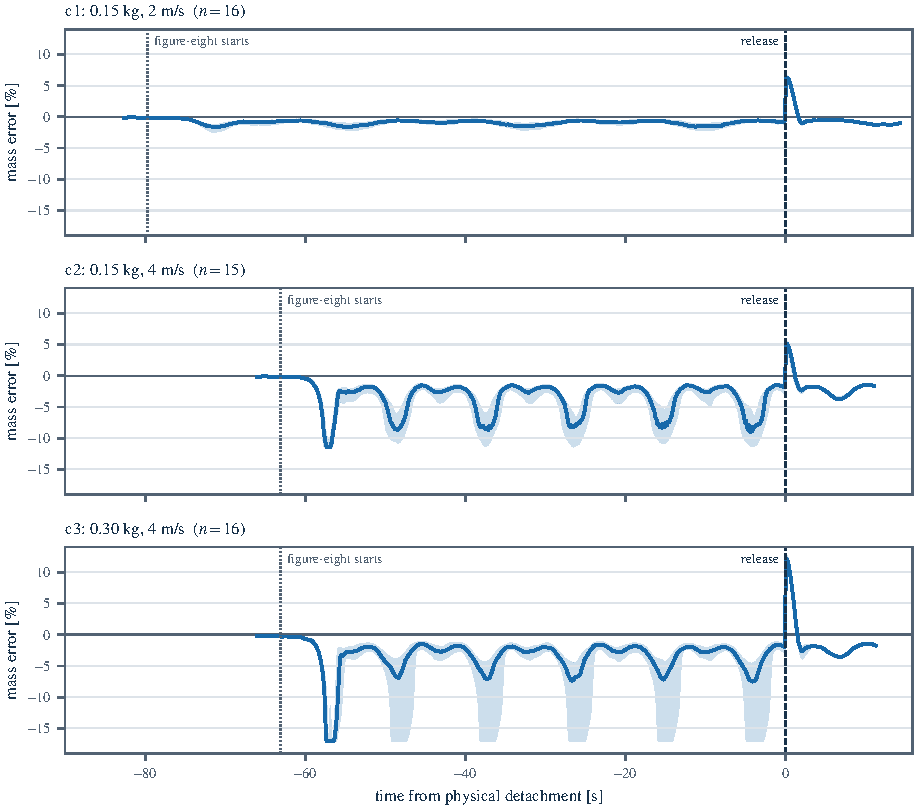
\includegraphics[width=0.98\textwidth]{Figures/fig_cohort_mass.pdf}
\caption[Composite-mass error through carry and release]{Composite-mass error $(\hat m-m)/m$ of the nominal (d0) cohort
flights, each aligned on its own physical detachment and scored against its own
truth. Line: median over flights; band: 10th--90th percentile. Traces start at
the end of the lift ramp, because before lift-off the parcel rests on the ground
and the joint record is not a usable truth. The positive transient at release is
the estimator's lag behind an instantaneous truth step. The floor of the c3 band
at \SI{-17}{\percent} is the mass lower bound $0.95\,\mB$.}
\label{fig:cohortmass}
\end{figure}

\begin{table}[ht]
\centering
\caption[Composite-mass error by flight phase]{Composite-mass error by flight phase, all physically attached cohort
flights (all arms and scenarios; the estimator is identical across arms).
Errors are medians over flights of the per-flight mean, with the range of
per-flight values in brackets; post-release error is relative to $\mB$.
Collapse fraction: share of loaded figure-eight samples with
$\hat m_P<\tfrac12 m_P$. Bound: share resting on $\mT=0.95\,\mB$.}
\label{tab:massbias}
\small
\begin{tabular}{@{}l c c c c c c@{}}
\toprule
\textbf{Cond.} & $n$ & \textbf{Hover [\%]} & \textbf{Figure-eight [\%]} &
\textbf{Post [\%]} & \textbf{Collapse} & \textbf{Bound} \\
\midrule
c1 & 40 & $-0.21$ & $-0.97$ [$-2.50$, $-0.47$] & $-0.94$ & 0.00 [0, 0.12] & 0.000 \\
c2 & 39 & $-0.22$ & $-4.09$ [$-6.27$, $-2.37$] & $-1.70$ & 0.38 [0.21, 0.73] & 0.010 \\
c3 & 39 & $-0.29$ & $-3.30$ [$-8.09$, $-1.62$] & $-1.68$ & 0.03 [0, 0.40] & 0.014 \\
\bottomrule
\end{tabular}
\end{table}

Three findings follow. First, in loaded hover the estimate is accurate in every
flight: the per-flight mean error lies between \SI{-0.44}{\percent} and
\SI{-0.10}{\percent} of the composite mass, which for the lighter payload is
within about \SI{10}{\gram}. No physically attached flight failed to recognise
its payload. Second, in the figure-eight the bias is small at
\SI{2}{\meter\per\second} (median \SI{-1.0}{\percent}) and roughly four times
larger at \SI{4}{\meter\per\second}, and it is not constant: the error dips
about once every \SI{11}{\second}, half the figure-eight period, to
\SIrange{-6}{-9}{\percent} in the median trace. The first dip, at the entry to
the figure-eight while the speed ramps up, takes the median of both
\SI{4}{\meter\per\second} conditions to the lower mass bound. Because the dip is
a fixed fraction of the composite mass, it is a larger fraction of the
\emph{payload} for the lighter one, which is why the collapse fraction is
highest at c2 (median $0.38$) although c3's dips reach the bound more often.
Third, after release the estimate settles slightly below the bare airframe,
\SIrange{-0.9}{-1.7}{\percent} of $\mB$; since $\hat m_P=(\hat m-\mB)^+$ is then
zero, the release confirmation is unaffected.

The manoeuvre-induced dips of the second finding are the collapse that
Section~\ref{sec:eval:limits} discusses as the dominant failure of the
interface. In the evaluated configuration the collapse fraction had medians of
$0$, $0.38$ and $0.03$
at c1, c2 and c3, with the per-flight maximum reaching $0.73$ at c2
(Table~\ref{tab:massbias}); at \SI{4}{\meter\per\second} the estimate touched
the mass lower bound at the entry to the figure-eight in at least half the
flights, and in some c3 flights at every dip thereafter
(Figure~\ref{fig:cohortmass}). Its lifecycle consequence is reported in
Section~\ref{sec:eval:unsignaled}. The collapse no longer cost a flight: the inertia
floor held the inner-loop scale at $2.34$ through every loaded figure-eight
(Section~\ref{sec:eval:opslimit}), the residual kept the vertical tracking
error below \SI{1}{\milli\meter} on average (Section~\ref{sec:eval:l1ablation}),
and no eligible flight diverged. But it was not prevented, and its effect on the
lifecycle is undiminished. Development flights that show the mechanism of the collapse, in earlier
configurations, are reported separately in Section~\ref{sec:eval:collapse}.

\subsection{Release completion and delay}\label{sec:eval:completion}

Two delay modes are possible by construction and would have to be reported
separately rather than pooled: confirmation while the vehicle is still flying
the figure-eight, and confirmation after the \SI{12}{\second} timeout has
declared \textsc{unresolved} and the vehicle has braked to hover. In the cohort
only the first occurred. Table~\ref{tab:completion} lists completion and delay
for every eligible flight.

\begin{table}[ht]
\centering
\caption[Release completion and confirmation delay]{Release completion and confirmation delay, all eligible cohort flights.
Delay is from the release command to acceptance; under delayed detachment (d4)
it is also given from the physical detachment. CP: two-sided
\SI{95}{\percent} Clopper--Pearson interval on the completion rate. Ranges are
over flights.}
\label{tab:completion}
\small
\begin{tabular}{@{}l c c c c c c@{}}
\toprule
\textbf{Cond.} & \textbf{Arm} & \textbf{Scen.} & \textbf{Done} & \textbf{CP} &
\textbf{From command [s]} & \textbf{From detachment [s]} \\
\midrule
c1 & A & d0 & 8/8 & [0.63, 1] & 0 & 0 \\
   & A & d4 & 8/8 & [0.63, 1] & 0 & $-4.08$ \\
   & B & d0 & 8/8 & [0.63, 1] & 2.96 (2.76--3.00) & 2.96 \\
   & B & d4 & 8/8 & [0.63, 1] & 7.16 (7.10--7.26) & 3.07 \\
   & C & d4 & 8/8 & [0.63, 1] & 7.13 (7.10--7.16) & 3.07 \\
\midrule
c2 & A & d0 & 7/7 & [0.59, 1] & 0 & 0 \\
   & A & d4 & 8/8 & [0.63, 1] & 0 & $-4.07$ \\
   & B & d0 & 8/8 & [0.63, 1] & 2.60 (2.30--2.70) & 2.60 \\
   & B & d4 & 8/8 & [0.63, 1] & 6.56 (6.30--6.76) & 2.51 \\
   & C & d4 & 8/8 & [0.63, 1] & 6.65 (6.40--6.76) & 2.62 \\
\midrule
c3 & A & d0 & 8/8 & [0.63, 1] & 0 & 0 \\
   & A & d4 & 8/8 & [0.63, 1] & 0 & $-4.03$ \\
   & B & d0 & 8/8 & [0.63, 1] & 3.03 (2.90--3.16) & 3.03 \\
   & B & d4 & 8/8 & [0.63, 1] & 7.10 (6.96--7.26) & 3.06 \\
   & C & d4 & 7/7 & [0.59, 1] & 7.00 (6.96--7.20) & 2.97 \\
\bottomrule
\end{tabular}
\end{table}

Every one of the $118$ eligible flights completed its release (CP interval
$[0.969, 1]$); none reached \textsc{unresolved}, and no flight diverged. Pooled
over conditions and scenarios, arm~B completed $48$ of $48$
($[0.926, 1]$). Arm~B's confirmation arrived \SIrange{2.3}{3.2}{\second} after
the payload physically left, in manoeuvre, with medians of \SI{3.0}{\second}
at \SI{2}{\meter\per\second} and \SIrange{2.5}{3.1}{\second} at
\SI{4}{\meter\per\second}. About \SI{1}{\second} of this is the persistence
hold of \eqref{eq:confirm}; the rest is the time the estimate takes to fall
through the evidence-score transition band (Figure~\ref{fig:cohortmass}). That delay is the
price of confirmation under nominal conditions, where the command is true.

The completion rate does not by itself show that the confirmations were
correct. Arm~B also confirmed releases that had not happened: $114$ times
during loaded carry, all at \SI{4}{\meter\per\second}, before any command.
These are reported with arm~C in Section~\ref{sec:eval:unsignaled}; arm~C
confirmed real detachments in the same \SIrange{2.4}{3.2}{\second} range
(Table~\ref{tab:completion}).

\subsection{Delayed detachment}\label{sec:eval:delayed}\label{sec:eval:paired}

A command-triggered arm accepts the release at the command and therefore
declares, for the whole of the hold, that a payload has gone which is still
attached. As Section~\ref{sec:eval:arms} explains, in the continuous interface
this does not put an empty model on the loaded vehicle: the controller's mass
and inertia keep following the estimate, which still sees the payload. What the
early acceptance does change is the lifecycle's report, which is wrong for the
duration of the hold, and the residual $\hat{\bm d}$, which is reset while the
mass bias it was compensating is still present. An evidence-gated arm should
accept in none of these flights.

That is what the cohort shows. Arm~A accepted before the joint was removed in
all $24$ of its delayed-detachment flights, about \SI{4.0}{\second} early in
each; arms~B and~C accepted early in none of their $47$
(Table~\ref{tab:completion}). Measured from the physical detachment, arm~B's
confirmation came \SIrange{2.3}{3.2}{\second} later (medians
\SIrange{2.5}{3.1}{\second}), the same as under nominal release: holding the
joint for \SI{4}{\second} neither produced a confirmation during the hold nor
slowed the one after it. What this experiment shows is a difference in
\emph{lifecycle correctness}. It does not show a difference in tracking or
survival, and none was expected with the hold this short and the mass model
unaffected; a permanently jammed gripper is a separate test.

\subsection{Command-armed versus always-on confirmation}\label{sec:eval:unsignaled}

A delayed-detachment result reflects \emph{persistent confirmation}: arm~C,
which starts counting only after the command, also never accepts early. The
difference between arms~B and~C lies elsewhere. Arm~B's confirmation rule runs
throughout loaded flight and can fire during carry if the mass estimate
collapses (Section~\ref{sec:frame:limits-lifecycle}); arm~C's cannot, because it
is not armed until the command. The comparison therefore measures what running
the rule before the command costs in false confirmations.

\begin{table}[ht]
\centering
\caption[Release confirmations during loaded carry]{Release confirmations during loaded carry (after physical attachment,
before the release command), all physically attached cohort flights.
Arm~A does not run the confirmation rule.}
\label{tab:carryconf}
\small
\begin{tabular}{@{}l c c c c@{}}
\toprule
\textbf{Cond.} & \textbf{B: flights} & \textbf{B: confirmations} &
\textbf{C: flights} & \textbf{C: confirmations} \\
\midrule
c1 & 0 of 16 & 0 & 0 of 8 & 0 \\
c2 & 14 of 16 & 78 & 0 of 8 & 0 \\
c3 & 6 of 16 & 36 & 0 of 7 & 0 \\
\bottomrule
\end{tabular}
\end{table}

Table~\ref{tab:carryconf} gives the result. Arm~C confirmed no release during
loaded carry in any of its $23$ flights, a per-flight rate whose
\SI{95}{\percent} upper bound is $0.15$. Arm~B confirmed $114$ releases that had
not happened, in $20$ of its $32$ flights at \SI{4}{\meter\per\second} and in
none of its $16$ at \SI{2}{\meter\per\second}. They are not isolated events: an
affected flight typically confirmed about six times, spaced about \SI{11}{\second}
apart, each time at an evidence score above $0.99$. The spacing is the half-period of
the figure-eight and coincides with the dips of Figure~\ref{fig:cohortmass}: each
dip carries $\hat m_P$ below the confirmation threshold for longer than the
\SI{1}{\second} hold. At c2 the light payload makes this nearly certain; at c3 the
same relative dip leaves more payload mass above the threshold, and it happened
in fewer flights.

In the evaluated configuration these false confirmations had no effect on
control. With no release command pending, an acceptance neither resets
$\hat{\bm d}$ nor ends the inertia floor, and the controller's mass follows the
estimate in either case; the release command re-arms the rule, so the genuine
release was still confirmed in every flight. The error is in the lifecycle's
report: a delivery system that acted on \emph{release confirmed} would, at
\SI{4}{\meter\per\second}, have been told repeatedly that a parcel still on the
hook had been delivered. Arm~C avoids this by construction, at no cost in delay
(Table~\ref{tab:completion}); its price is that it cannot detect a release that
was never commanded.

The comparison settles the arming policy. The always-on rule of arm~B is a
negative result: it shows that, in this configuration, mass evidence alone does
not separate a loaded vehicle in manoeuvre from an empty one, and a rule that
admits only that evidence will accept releases that have not happened. The
command-armed rule of arm~C keeps the property the delayed-detachment experiment
established --- it does not accept a release while the payload is still
attached --- without the false acceptances, and without a longer delay after
detachment. It is the mechanism the present evidence supports. Its scope is
correspondingly narrower: it distinguishes a commanded release from a physical
detachment, and it cannot by itself detect a load lost without a command.

\subsection{Tracking performance}\label{sec:eval:nominal}

Under nominal conditions the command is true, so waiting for confirmation can
gain nothing and costs a delay; arm~A has zero confirmation delay by
construction. The purpose of the nominal pairs is to establish that the
always-on confirmed arm completes and tracks as well as the command-triggered
one, not that it is better: in the continuous interface the controller's mass
and inertia follow the estimate in both arms, so no tracking difference is
expected.

Pairs are formed within a block at the same condition. Both arms completed
every pair. Post-release position RMSE (median over pairs, arm~A against
arm~B) was \SI{0.028}{\meter} against \SI{0.026}{\meter} at c1 ($n=8$,
Wilcoxon $p=0.38$), \SI{0.108}{\meter} against \SI{0.088}{\meter} at c2
($n=7$, $p=0.078$) and \SI{0.104}{\meter} against \SI{0.102}{\meter} at c3
($n=8$, $p=0.74$). Loaded figure-eight RMSE, before any difference between the
arms can act, was \SIrange{0.029}{0.033}{\meter} at c1 and
\SIrange{0.118}{0.126}{\meter} at \SI{4}{\meter\per\second} in both arms. No
difference in post-release stability was detected; the c2 pair count is seven
because one arm~A flight missed its grasp (Table~\ref{tab:attempts}).

Tracking is therefore governed by the condition rather than by the release arm:
loaded figure-eight RMSE is about \SI{0.03}{\meter} at \SI{2}{\meter\per\second}
and about \SI{0.12}{\meter} at \SI{4}{\meter\per\second}. What does change
tracking is the residual specific force, whose contribution is isolated in
Section~\ref{sec:eval:l1ablation}.

\section{Historical Release Campaign with Force-Balance Evidence}\label{sec:eval:campaign}

This campaign was flown with the full-state estimator F from the campaign code
base, before the reduced estimator was adopted. Its release, fault and
thrust-map experiments were repeated with the deployed system in
Section~\ref{sec:eval:deployed}, whose results supersede these for the deployed
system; the controller comparison of Section~\ref{sec:eval:camp:ctrl} exists
only here. The cohort leaves three questions open: whether release evidence that does not
pass through the mass estimate removes the carry-phase false acceptances of the
always-on rule; whether such a rule can detect a load lost without a command and
remain safe when a commanded release fails; and how the interface compares with
fixed-parameter and lumped-adaptive control. A second frozen campaign of $312$
flights, run on 3--4~November~2026, addresses them with the force-balance rule
of Section~\ref{sec:frame:accdet}, here called arm~D. Its results are reported
separately from the cohort and are not pooled with it; the earlier cohort's logs
were used only for offline replay before the campaign was frozen.

\subsection{Design}\label{sec:eval:camp:design}

Arm~D is the dual-enabled force-balance rule: the score \eqref{eq:gammaacc},
consumed only when a release command is pending or the uncommanded-loss
watchdog is armed. Arm~A is the command-immediate arm of Table~\ref{tab:arms}.
The two arms share every other setting of the evaluated configuration of
Section~\ref{sec:eval:config}, and they differ only in the release lifecycle.
A fourth condition, c4 (\SI{0.30}{\kg} at \SI{2}{\meter\per\second}), completes
a two-by-two mass--speed design with c1--c3 as defined in
Section~\ref{sec:eval:conditions}. Table~\ref{tab:camp-design} lists the four
experiments.

\begin{table}[ht]
\centering
\caption[Experiments of the force-balance release campaign]{Experiments of the
force-balance release campaign. All four conditions c1--c4 appear in every
experiment. d0: nominal release; d4: detachment held \SI{4}{\second} after the
command.}
\label{tab:camp-design}
\small
\begin{tabularx}{\textwidth}{@{}l c >{\raggedright\arraybackslash}X >{\raggedright\arraybackslash}p{0.17\textwidth}@{}}
\toprule
\textbf{Experiment} & \textbf{Flights} & \textbf{Factors} & \textbf{Arm} \\
\midrule
E1 Release semantics & 144 & arm A/D $\times$ d0/d4 $\times$ 4 conditions; 9 paired blocks & A and D \\
E2 Controller comparison & 72 & Fixed / $\mathcal{L}_1$ / MHE $\times$ 4 conditions; 6 rounds; d0 & D \\
E3 Thrust-map error & 48 & detector thrust scaled by $0.90$ / $1.10$ $\times$ 4 conditions; 6 rounds; d0 & D \\
E4 Faults & 48 & uncommanded loss / jammed gripper $\times$ 4 conditions; 6 rounds & D \\
\bottomrule
\end{tabularx}
\end{table}

In E1 each block contains one round of eight flights with nominal release and
one with delayed detachment, both rounds covering the four conditions under
both arms, with the order of the rounds and of the flights within them drawn
from a recorded seed. In E2 the three controllers share the arm-D lifecycle,
the inertia floor and the inner-loop scheduling, and differ only in their
translational compensation. \emph{Fixed} keeps the bare-airframe mass in the
prediction model with no translational adaptation. \emph{$\mathcal{L}_1$} keeps
the same mass and compensates with the residual $\hat{\bm d}$ alone. \emph{MHE}
is the evaluated configuration, with the estimated mass and $\hat{\bm d}$. E3
models a miscalibrated thrust coefficient $k_f$ on the estimation side: the thrust
reconstructed from rotor speeds is scaled by a fixed factor in both of its
consumers, the estimator's thrust input and the thrust \eqref{eq:macc} of the
force-balance detector. The plant's rotor coefficient, the controller's
thrust-to-throttle map and the thrust used by the residual $\hat{\bm d}$ keep the
nominal $k_f$. The payload mass and thresholds are not altered, and the factor
actually applied is recorded in the estimator's and the controller's log of
every flight ($0.900$ and $1.100$ in $24$ flights each). Because the estimated
mass enters the controller's model, the error also reaches the control input,
through the mass estimate. In E4 an \emph{uncommanded loss} detaches the payload at the
release phase with no command, no pending release and no notification to the
estimator. A \emph{jammed gripper} receives the normal command and never
releases.

Thresholds, filters, arming and confirmation times, controller and trajectory
parameters were frozen before the first flight. A fingerprint of the flight code
was recorded at the start and checked before every flight; it did not change.
A flight was eligible if the payload physically attached, the vehicle survived
to the release command or the injected fault, the estimator, controller,
gripper, inertial, rotor-speed and residual logs were complete, and the
recorded configuration matched the schedule. False or missed confirmations,
divergence, solver failures, large tracking errors, an \textsc{unresolved}
jam and a failed recovery after loss count as results, never as exclusions; in
E2 a divergence before the command counts as a controller failure. Ineligible
flights would have been replaced, and only those; none occurred. All $312$
scheduled flights attached and were eligible, so every cell has its planned size
(nine per E1 cell, six per cell elsewhere). No flight in the campaign diverged.
Post-release metrics here use a window from physical detachment (or the
injected loss) to \SI{25}{\second} after it, which differs from the cohort's
window; post-release numbers are not comparable across the two.

\subsection{Release semantics and carry-phase acceptance}\label{sec:eval:camp:release}

\begin{table}[ht]
\centering
\caption[Release acceptance under the force-balance rule (E1)]{Release
acceptance under the force-balance rule (E1). Median (range) over nine flights
per cell. det.: time of acceptance relative to physical detachment (negative =
before the payload left); cmd: relative to the release command.
Every flight in every cell completed its release.}
\label{tab:camp-release}
\small
\begin{tabular}{@{}l c c c c@{}}
\toprule
& \textbf{A, d4} & \textbf{D, d0} & \multicolumn{2}{c}{\textbf{D, d4}} \\
\cmidrule(lr){2-2}\cmidrule(lr){3-3}\cmidrule(lr){4-5}
\textbf{Cond.} & \textbf{det.\ [s]} & \textbf{det.\ [s]} &
\textbf{cmd [s]} & \textbf{det.\ [s]} \\
\midrule
c1 & $-4.05$ ($-4.09$ to $-4.04$) & 2.06 (2.00--2.15) & 6.20 (6.10--6.26) & 2.12 (2.05--2.21) \\
c2 & $-4.09$ ($-4.10$ to $-4.04$) & 1.94 (1.90--2.05) & 6.10 (6.00--6.16) & 2.01 (1.91--2.12) \\
c3 & $-4.09$ ($-4.09$ to $-4.00$) & 2.30 (2.20--2.44) & 6.40 (6.25--6.45) & 2.31 (2.20--2.44) \\
c4 & $-4.05$ ($-4.09$ to $-4.04$) & 2.40 (2.30--2.46) & 6.46 (6.34--6.60) & 2.41 (2.34--2.51) \\
\bottomrule
\end{tabular}
\end{table}

Table~\ref{tab:camp-release} reproduces the delayed-detachment result of the
cohort with the new evidence. Arm~A accepted before the payload left in all
$36$ of its delayed-detachment flights, by \SI{4.05}{\second} at the median.
Arm~D accepted early in none of its $36$ (\SI{95}{\percent} CP upper bound
$0.10$) and completed all $72$ of its releases ($[0.950, 1]$). Its confirmation
came \SIrange{1.90}{2.51}{\second} after physical detachment (median
\SI{2.20}{\second}, 95th percentile \SI{2.44}{\second}). Holding the joint for
\SI{4}{\second} did not change the delay measured from detachment. About
\SI{1}{\second} of it is the persistence hold; the rest is the two low-pass
stages of \eqref{eq:macc}--\eqref{eq:gammaacc}.

The delay depends on the mass and hardly at all on the speed. In an
effect-coded two-by-two regression on the nominal flights, the heavier payload
lengthened the delay from detachment by \SI{0.35}{\second} ($\pm0.02$,
$p<10^{-15}$), the higher speed shortened it by \SI{0.08}{\second}
($p=0.0006$), and the interaction was not detectable ($+0.02$, $p=0.64$); under
delayed detachment the effects were $+0.30$, $-0.14$ and $+0.01$\,s ($p=0.76$
for the interaction). A larger payload leaves a larger step for the filtered
score to traverse before it crosses $0.90$.

The comparison that matters for the arming policy is carry. In every arm-D
flight the watchdog armed after the lift and before the release command, a
median of \SI{3.2}{\second} after the start of the lift (range
\SIrange{1.9}{3.9}{\second}). From that point, the rule was able to accept a
release at any time during carry, which is the always-on property that produced
the cohort's $114$ false acceptances. Across all $240$ flights of the campaign
flown with the arm-D lifecycle, the watchdog was armed in $228$, and no release
was accepted during loaded carry in any flight (\SI{95}{\percent} upper bound
$0.016$ per armed flight), including every armed flight at c2, the condition
at which the mass evidence had failed in $14$ of $16$ cohort flights. The force balance
therefore separates a loaded vehicle in manoeuvre from an empty one where the
mass estimate did not. The twelve flights in which the watchdog did not arm are
the thrust-map cases of Section~\ref{sec:eval:camp:thrust}.

Arm~D's delay after detachment, \SIrange{1.9}{2.5}{\second}, is also shorter
than the \SIrange{2.3}{3.2}{\second} of the cohort's mass-evidence arms. The two
come from different batches and are not a paired comparison.

Tracking did not differ consistently between the arms. Of the eight within-block
pairings of post-release RMSE (four conditions, two scenarios), seven showed no
difference ($p\ge0.07$, Wilcoxon, nine pairs each); at c3 with delayed
detachment arm~D's was higher by \SI{0.014}{\meter} at the median ($p=0.004$).
As in the cohort, the result concerns the lifecycle, not tracking.

\subsection{Uncommanded loss and a jammed gripper}\label{sec:eval:camp:loss}

\begin{table}[ht]
\centering
\caption[Faults under the force-balance rule (E4)]{Faults under the
force-balance rule (E4), six flights per cell. Loss: payload detached with no
command. Armed: watchdog armed before the loss. Delay: from detachment to the
declared loss, median (range). Reset: geometry zeroed and inner-loop scale
returned to the bare airframe. Jam: command issued, payload never released.
False acc.: release accepted. Hover: \textsc{unresolved}, braked, then hovering
below \SI{0.5}{\meter\per\second}.}
\label{tab:camp-loss}
\small
\begin{tabular}{@{}l c c c c c c@{}}
\toprule
& \multicolumn{4}{c}{\textbf{Uncommanded loss}} & \multicolumn{2}{c}{\textbf{Jammed gripper}} \\
\cmidrule(lr){2-5}\cmidrule(lr){6-7}
\textbf{Cond.} & \textbf{Armed} & \textbf{Detected} &
\textbf{Delay [s]} & \textbf{Reset} & \textbf{False acc.} &
\textbf{Hover} \\
\midrule
c1 & 6/6 & 6/6 & 2.03 (1.76--2.10) & 6/6 & 0/6 & 6/6 \\
c2 & 6/6 & 6/6 & 1.94 (1.90--2.00) & 6/6 & 0/6 & 6/6 \\
c3 & 6/6 & 6/6 & 2.34 (2.20--2.50) & 6/6 & 0/6 & 6/6 \\
c4 & 6/6 & 6/6 & 2.38 (2.30--2.46) & 6/6 & 0/6 & 6/6 \\
\bottomrule
\end{tabular}
\end{table}

Table~\ref{tab:camp-loss} gives the fault results. The watchdog was armed
before the loss in all $24$ uncommanded-loss flights, and every loss was
detected ($24/24$, $[0.86, 1]$), \SIrange{1.8}{2.5}{\second} after the payload
left; none was declared before it. In every case the payload geometry was
zeroed, the inner-loop scale returned from the floor value to that of the bare
airframe, no planned release was issued afterwards, and no flight diverged;
the largest post-loss position error had a median between \SI{0.08}{\meter} and
\SI{0.20}{\meter} by condition. This is the scenario the cohort could not fly,
because under the mass-evidence rules nothing other than the command ended the
inertia floor (Section~\ref{sec:eval:conditions}).

The jammed gripper is the converse test: the command is true and the
detachment never comes. No release was accepted in any of the $24$ flights
($0/24$, $[0, 0.14]$), and the payload model was never cleared. Every flight
reached \textsc{unresolved} at the \SI{12}{\second} timeout, armed the braking
reference and came to hover, with a largest speed in hover of
\SI{0.18}{\meter\per\second} over all flights.

\subsection{Thrust-map error}\label{sec:eval:camp:thrust}

\begin{table}[ht]
\centering
\caption[Estimation-side thrust-map error (E3)]{Estimation-side thrust-map
error (E3), applied to the estimator and the force-balance detector together;
detector quantities shown, six flights per cell. $m_{\mathrm{acc}}$
bias: median error relative to the true composite mass, in loaded carry and
after release. $\gamma_{\mathrm{acc}}$ max: median over flights of the largest
score in loaded carry. Delay from the command.}
\label{tab:camp-thrust}
\small
\begin{tabular}{@{}l l c c c c c c@{}}
\toprule
\textbf{Gain} & \textbf{Cond.} & \textbf{Bias, carry} & \textbf{Bias, post} &
$\gamma_{\mathrm{acc}}$ \textbf{max} & \textbf{Armed} & \textbf{Done} &
\textbf{Delay [s]} \\
\midrule
0.90 & c1 & $-10.4\,\%$ & $-10.3\,\%$ & 1.00 & 0/6 & 6/6 & 0.96 \\
     & c2 & $-10.7\,\%$ & $-10.5\,\%$ & 1.00 & 0/6 & 6/6 & 0.95 \\
     & c3 & $-10.7\,\%$ & $-10.6\,\%$ & 0.62 & 6/6 & 6/6 & 1.48 \\
     & c4 & $-10.4\,\%$ & $-10.4\,\%$ & 0.18 & 6/6 & 6/6 & 1.56 \\
\midrule
1.10 & c1 & $+9.3\,\%$ & $+9.8\,\%$ & 0.00 & 6/6 & 0/6 & --- \\
     & c2 & $+9.1\,\%$ & $+9.8\,\%$ & 0.00 & 6/6 & 0/6 & --- \\
     & c3 & $+9.0\,\%$ & $+9.8\,\%$ & 0.00 & 6/6 & 0/6 & --- \\
     & c4 & $+9.3\,\%$ & $+9.8\,\%$ & 0.00 & 6/6 & 0/6 & --- \\
\bottomrule
\end{tabular}
\end{table}

The force-balance mass moved one-for-one with the injected error
(Table~\ref{tab:camp-thrust}), and the two directions failed differently, as
the analysis of Section~\ref{sec:eval:thrustcal} predicts for the mass channel.
A \SI{10}{\percent} error in the composite mass is \SIrange{0.22}{0.24}{\kg},
larger than the lighter payload and close to the heavier one.

\emph{Overestimated thrust ($1.10$).} After release the empty vehicle read about
\SI{10}{\percent} heavier than it was, the score never rose, and none of the
$24$ releases was confirmed. Every flight reached \textsc{unresolved}, braked and
hovered, without divergence. The failure is a miss, and it ends in the safe
state the timeout was designed for. By the same arithmetic, an uncommanded loss
would also go undetected; that was not flown.

\emph{Underestimated thrust ($0.90$).} No release was accepted during carry and
every release completed, faster than nominally. That outcome hides two
failures. With the lighter payload the loaded vehicle already read as empty
--- the score was $1.00$ throughout carry --- so the watchdog never armed in any
of the $12$ flights: protection against uncommanded loss was silently lost.
Confirmation followed the command by the length of the hold alone, because the
score was already high; with delayed detachment, which E3 did not include, the
same rule would be expected to accept before the payload left. The deployed-system
validation flew that combination, and the rule did accept early in every flight
(Section~\ref{sec:eval:deployed}). With the heavier
payload the watchdog armed, but the largest carry score reached $0.85$ in one
flight, close to the $0.90$ threshold. The dual enabling prevented every false
acceptance in E3; it cannot restore evidence the thrust map has removed.

\emph{The estimator's mass.} The same error reached the controller's model
through the estimate. During loaded carry (from \SI{5}{\second} after lift to the
command), the median mass in the controller's model was
\SIrange{7.4}{9.2}{\percent} above truth with the map $1.10$. With the map $0.90$
it stayed at the bare-airframe value in all four conditions (cell medians
\SIrange{2.064}{2.076}{\kg}, against \SI{2.214}{\kg} and \SI{2.364}{\kg} of truth):
the payload was never recognised in the controller's model. This is the first of
the two failures predicted in Section~\ref{sec:eval:thrustcal}, and the replay of
Section~\ref{sec:eval:reduced} shows the full-state estimate pressed against its
$0.95\,\mB$ bound in this case. None of the $48$ flights of E3 diverged.

\subsection{Fixed, $\mathcal{L}_1$ and MHE controllers}\label{sec:eval:camp:ctrl}

\begin{table}[ht]
\centering
\caption[Controller comparison under the force-balance rule (E2)]{Controller
comparison under the force-balance rule (E2), nominal release. Medians over six
flights per cell. Loaded RMSE: from \SI{5}{\second} into the figure-eight to the
command. Post: detachment to \SI{25}{\second} after it. Delay from detachment.}
\label{tab:camp-ctrl}
\small
\begin{tabular}{@{}l l c c c c@{}}
\toprule
\textbf{Cond.} & \textbf{Controller} & \textbf{Loaded RMSE [m]} &
\textbf{Post RMSE [m]} & \textbf{Post peak [m]} & \textbf{Delay [s]} \\
\midrule
c1 & Fixed & 0.087 & 0.031 & 0.090 & 2.00 \\
   & $\mathcal{L}_1$ & 0.032 & 0.030 & 0.077 & 2.03 \\
   & MHE   & 0.033 & 0.026 & 0.072 & 2.08 \\
\midrule
c2 & Fixed & 0.151 & 0.118 & 0.203 & 1.94 \\
   & $\mathcal{L}_1$ & 0.099 & 0.085 & 0.136 & 2.02 \\
   & MHE   & 0.123 & 0.102 & 0.163 & 1.97 \\
\midrule
c3 & Fixed & 0.218 & 0.130 & 0.211 & 2.25 \\
   & $\mathcal{L}_1$ & 0.114 & 0.107 & 0.198 & 2.29 \\
   & MHE   & 0.117 & 0.096 & 0.206 & 2.32 \\
\midrule
c4 & Fixed & 0.168 & 0.036 & 0.170 & 2.40 \\
   & $\mathcal{L}_1$ & 0.030 & 0.045 & 0.149 & 2.40 \\
   & MHE   & 0.028 & 0.033 & 0.134 & 2.40 \\
\bottomrule
\end{tabular}
\end{table}

All $72$ flights completed their release without divergence or saturation of
the collective thrust, with one solver failure in one flight, and the
confirmation delay did not depend
on the controller (Table~\ref{tab:camp-ctrl}). Flights were paired within
rounds; with six pairs the smallest attainable two-sided Wilcoxon $p$ is
$0.031$.

Against the fixed-parameter controller the benefit of adaptation is clear in
loaded carry: the MHE controller had the smaller loaded RMSE in all $24$ pairs
($p=0.031$ in each condition), by \SIrange{0.04}{0.14}{\meter} at the median,
largest with the heavier payload. After release, when the fixed model is again
correct, the difference in RMSE shrank to \SIrange{0.002}{0.033}{\meter} and
was consistent only at c1 ($p=0.031$).

Against the $\mathcal{L}_1$ controller, which compensates the same payload with
the residual alone, no consistent difference in loaded tracking was found
($p\ge0.16$ in every condition); at c2 the $\mathcal{L}_1$ controller was
nominally the better in five of six pairs. After release the MHE controller had
the smaller peak error at both \SI{2}{\meter\per\second} conditions in all six
pairs ($p=0.031$), by \SIrange{0.006}{0.017}{\meter}, and the smaller RMSE at
c4 ($p=0.031$); at \SI{4}{\meter\per\second} there was no consistent
difference. With the residual present in both, estimating the mass is therefore
not shown to improve tracking in carry, and its measurable effect in this
experiment is a small one in the transient after release at low speed. The
three controllers also share the inertia floor and the inner-loop scheduling, so
E2 does not test the rotational benefit of the payload model.

\subsection{Scope of the campaign}\label{sec:eval:camp:limits}

The campaign has the limitations of the cohort --- simulation only, one
airframe and gripper geometry, centred grasps, no wind --- and some of its own.
The thrust-map error was applied to the estimator and the detector together.
The plant, the controller's thrust-to-throttle map and the residual were not
perturbed, so E3 does not represent an error that also affects the actuation
side. E3 also used only nominal release; delayed detachment with an
under-reading map was flown later, with the deployed system
(Section~\ref{sec:eval:deployed}). Every zero-count result is bounded by the cell sizes: an upper bound of
$0.10$ for early acceptance and $0.14$ for false acceptance under a jam. The
interface code of the campaign was not committed; the record holds the base
revision, a patch of the uncommitted changes and an archive of untracked files,
as for the cohort (Section~\ref{sec:eval:repro}). The campaign's data and scoring
scripts are in \texttt{release\_paper\_20261103\_210022/}.

\section{Ablations}\label{sec:eval:ablations}

\subsection{The residual specific force}\label{sec:eval:l1ablation}

The residual $\hat{\bm d}$ of Section~\ref{sec:model:residual} is part of the
evaluated configuration, and its contribution was isolated in a separate frozen
batch of $48$ flights run on 1~November~2026 (block seed $1793469773$). Arm~B of
the cohort was flown with the residual on and off, everything else in the
evaluated configuration unchanged; the flight records confirm that the residual
switch is the only setting that differs between the two arms. Nominal release
(d0) was crossed with the three conditions, eight blocks each, in an order drawn
from the seed. The endpoints were fixed before the batch: primary, loaded
figure-eight position RMSE and mean vertical error; secondary, post-release
RMSE, completion, divergence, mass bias and confirmations during carry. All
$48$ flights attached, completed their release and did not diverge.

\begin{table}[ht]
\centering
\caption[Residual specific force on against off]{Residual specific force on against off (arm~B, nominal release).
Medians over eight within-block pairs per condition; ``better'' counts the pairs
in which the residual-on flight had the smaller value (for the vertical error,
the smaller magnitude); $p$: Wilcoxon signed-rank. Vertical error is
$z-z^{\mathrm{ref}}$ averaged over loaded figure-eight.}
\label{tab:l1ablation}
\small
\begin{tabular}{@{}l l c c c c@{}}
\toprule
\textbf{Metric} & \textbf{Cond.} & \textbf{On} & \textbf{Off} &
\textbf{Better} & $p$ \\
\midrule
Loaded figure-eight RMSE [m] & c1 & 0.033 & 0.047 & 8/8 & 0.008 \\
                             & c2 & 0.116 & 0.148 & 7/8 & 0.016 \\
                             & c3 & 0.106 & 0.145 & 8/8 & 0.008 \\
\midrule
Mean vertical error [mm]     & c1 & $+0.4$ & $-4.5$ & 7/8 & 0.008 \\
                             & c2 & $-0.8$ & $-28.4$ & 8/8 & 0.008 \\
                             & c3 & $+0.2$ & $-44.3$ & 8/8 & 0.008 \\
\midrule
Post-release RMSE [m]        & c1 & 0.023 & 0.044 & 8/8 & 0.008 \\
                             & c2 & 0.089 & 0.132 & 7/8 & 0.016 \\
                             & c3 & 0.073 & 0.115 & 8/8 & 0.008 \\
\bottomrule
\end{tabular}
\end{table}

Table~\ref{tab:l1ablation} gives the result. Without the residual the vehicle
flies the loaded figure-eight below its reference, by \SI{4.5}{\milli\meter} at
c1 and by \SI{28}{\milli\meter} and \SI{44}{\milli\meter} at the two
\SI{4}{\meter\per\second} conditions; with it the mean vertical error is under
\SI{1}{\milli\meter} at every condition. Loaded figure-eight RMSE falls by
\SIrange{22}{31}{\percent} and post-release RMSE by \SIrange{33}{48}{\percent},
in $23$ of the $24$ pairs on each metric. The sag grows with the
manoeuvre-induced mass bias of Section~\ref{sec:eval:estimation}, which is the
error the residual is there to absorb: an estimate that is low by a few percent
asks for a thrust that is low by the same fraction.

Equally informative is what the residual did not change. The loaded
figure-eight mass bias was the same in both arms (medians \SI{-0.9}{\percent}
against \SI{-0.8}{\percent}, \SI{-3.6}{\percent} against \SI{-3.1}{\percent},
\SI{-3.1}{\percent} against \SI{-3.5}{\percent}; all $p>0.19$), and so were the
confirmation delays (all $p>0.45$) and the confirmations during carry, which
occurred in both arms at c2. The residual compensates the \emph{consequence} of
the mass bias for tracking; it does not reduce the bias, and it does not touch
the lifecycle.

\subsection{Full-state versus reduced estimator}\label{sec:eval:reduced}

Every historical flight reported so far in this chapter was flown with the
full-state estimator F of Section~\ref{sec:model:mhe}. The deployed default is now the
reduced velocity--mass estimator R of Section~\ref{sec:frame:redmodel}. This
subsection gives the evidence for that change in three parts: an offline replay
over the recorded release campaign, a four-flight thrust-map smoke test of R in
closed loop, and a paired closed-loop comparison of F and R. The two estimators
share horizon, sampling, alignment of inputs and measurements, the velocity,
noise and arrival weights \eqref{eq:Wred}, initialisation and event logic; they
differ only in model structure and in the mass bound and health check of
Section~\ref{sec:frame:health}.

\paragraph{Offline replay.} R was solved offline on the odometry, the
interval-averaged reconstructed thrust and the \SI{10}{\hertz} solve instants of
all 312 flights of Section~\ref{sec:eval:campaign}, and compared with the
estimate F produced online in the same flights. The replay used F's lower bound
$0.95\,\mB$, so that only the model differs. Loaded windows run from
\SI{5}{\second} after lift-off to the command or detachment, post-release windows
from \SI{5}{\second} after detachment; convergence is entry into a
\SI{\pm0.03}{\kg} band held for \SI{1}{\second}.
Table~\ref{tab:reducedreplay} gives the flight-level medians for the 264 flights
with a nominal thrust map.

\begin{table}[ht]
\centering
\caption{Replay of the reduced estimator on the 264 nominal-thrust flights of the
release campaign, against the full-state estimate recorded online in the same
flights. Flight-level medians; paired Wilcoxon signed-rank tests.}
\label{tab:reducedreplay}
\small
\begin{tabular}{@{}lrrrr@{}}
\toprule
Metric & F (online) & R (replay) & R better & $p$ \\
\midrule
Loaded mass MAE [\si{\kg}] & 0.0359 & 0.0127 & 264/264 & $5\times10^{-45}$ \\
Post-release mass MAE [\si{\kg}] & 0.0291 & 0.0093 & 240/240 & $4\times10^{-41}$ \\
Convergence after lift-off [\si{\second}] & 4.21 & 4.22 & --- & --- \\
Return to the empty value within the flight & 183/240 & 240/240 & --- & --- \\
Solve time, median [\si{\milli\second}] & 2.8 & 0.16 & 264/264 & --- \\
\bottomrule
\end{tabular}
\end{table}

The reduced estimate was more accurate in every loaded and every post-release
window. Convergence after lift-off was unchanged. After release, 57 of the 240
full-state estimates never re-entered the band within the flight. All 57 were at
\SI{4}{\meter\per\second}, and they had not stalled: they settled
\SI{2.15}{\percent} below the empty value (median; interquartile range
\SIrange{-2.21}{-2.09}{\percent}) in the continuing figure-eight, which is outside
the band. The reduced estimate re-entered it in every flight. The solve times are indicative only: the replay ran on an otherwise
idle core and the online figure is a window mean.

Under the thrust-map error of Section~\ref{sec:eval:camp:thrust} the replay
behaved as the analysis of Section~\ref{sec:frame:health} predicts. With a map
\SI{10}{\percent} high the reduced estimate was biased high by the same
proportion (loaded MAE \SI{0.207}{\kg}, against \SI{0.198}{\kg} for F). With a
map \SI{10}{\percent} low it was driven onto the $0.95\,\mB$ bound: 107 of its
solves, in 22 of the 24 flights, ended at the iteration limit, all at or near
the bound. These 107 solves are \SI{0.03}{\percent} of all replay solves, but
they are the reason the deployed reduced estimator replaces the hard physical
bound by a wide numerical box and an explicit health check.

The replay has three limitations. It cannot measure tracking, because the
trajectories were generated with F in the loop. It uses the simulator's
near-ideal odometry. And it does not reproduce the grasp gap of
Section~\ref{sec:frame:gate}: it treats the logged solve instants as
consecutive, so the windows that span the gap join samples taken about
\SI{6}{\second} apart, and its lift-off convergence times are not a model of the
online ones. It supports the
reduced model as a mass estimator; it does not by itself justify putting it in the
loop.

\paragraph{Thrust-map smoke test.} Before the closed-loop comparison, R was flown
once in each of four conditions --- thrust map \SI{-10}{\percent} and
\SI{+10}{\percent}, payload \SI{0.15}{\kg} and \SI{0.30}{\kg}, at
\SI{2}{\meter\per\second} with immediate detachment --- with the pre-specified
rule that any divergence, any model update during an unhealthy interval or any
failed safety fallback would stop the comparison. None occurred. No flight
recorded a non-zero solver status or a re-initialisation, so the iteration-limit
failures of the replay did not recur with the wider box. In both \SI{-10}{\percent}
flights the estimate was \SIrange{10.2}{10.6}{\percent} low and was flagged below
the health band whenever the airframe was empty; the controller then held its
model, and its model mass did not change at all during any unhealthy interval.
Both releases were confirmed, and the controller's model returned to within
\SI{0.01}{\kg} of the empty value. With \SI{+10}{\percent} both
releases ended in \textsc{unresolved}, the expected outcome because the
over-reading thrust map makes the empty airframe look loaded, and both flights
braked to a safe hover. With the heavier payload the estimate left the band
upward during lift-off and the controller held, for the whole carry, the last
accepted value of \SI{2.272}{\kg} against a true \SI{2.364}{\kg}. That value is
closer to the truth than the \SI{2.60}{\kg} the estimator itself reported, but
it is whatever the estimate happened to be when it crossed the band edge during a
transient: the check prevents an implausible model, it does not supply a correct
one. With the lighter payload the \SI{+10}{\percent} estimate stayed inside the
band and was used.

\paragraph{Paired closed-loop comparison.} The deciding experiment flies F and R
in the same conditions with everything else frozen: release arm D, the
deployed controller, trajectory, gripper geometry, lifecycle and safety settings
of Section~\ref{sec:eval:campaign}, nominal thrust map, no injected fault. The
design crosses payload (\SI{0.15}{\kg}, \SI{0.30}{\kg}), speed
(\SI{2}{\meter\per\second}, \SI{4}{\meter\per\second}) and detachment (immediate,
\SI{4}{\second} after the command) with six paired replicates, $2\times2\times2\times6$
pairs and 96 flights. Within each of six blocks the eight cells are flown in
random order with the two estimators of a pair adjacent, in random order. Only
infrastructure failures are excluded; divergence, solver failure, early or
missed confirmation and \textsc{unresolved} are outcomes. Metrics, statistics
and the acceptance criteria were fixed before the first flight: paired
differences R$-$F with bootstrap confidence intervals of the median and Wilcoxon
signed-rank tests, by payload, speed and detachment as well as overall.

\paragraph{Execution.} The batch was flown on 5 and 6 November 2026 from a
recorded seed. Three deviations are recorded with it, none of which touches the
comparison. After flight~12 the experiment entry points changed their default
estimator; no flight reads that default, because every flight sets the variant
explicitly, but the change altered the code fingerprint, so the batch stopped
itself by design and was resumed under the new fingerprint. After flight~32, at a
block boundary, the batch was paused, and it was resumed the next day with the
fingerprint unchanged. All $96$ flights attached and were eligible, no
infrastructure rerun was needed, and all $48$ pairs are complete.

\paragraph{Binary outcomes.} Neither arm diverged, confirmed a release early,
missed one or entered \textsc{unresolved}; every release was confirmed and the
controller's model returned to the empty airframe afterwards, $48$ of $48$ in each
arm. F ended $14$ solves at the iteration limit and re-initialised its window
twice; R had no non-zero solver status. Under the nominal thrust map R's
mass-health check never flagged an estimate. The controller held its model for
\SI{8.7}{\second} with R and \SI{9.1}{\second} with F per flight at the median,
almost all of it in the grasp gap of Section~\ref{sec:frame:gate}, and its model
mass did not change during any hold.

\begin{table}[ht]
\centering
\caption[Full-state against reduced estimator in closed loop]{Full-state (F)
against reduced (R) estimator in closed loop, pre-specified metrics, all $48$
pairs. Medians per arm; $\Delta$ is the median paired difference R$-$F with its
bootstrap \SI{95}{\percent} confidence interval; $p$: Wilcoxon signed-rank;
B/S/W: pairs in which R was better, the same or worse. Loaded window: from
\SI{5}{\second} after lift-off to the command; post-release: from \SI{5}{\second}
after detachment to the end of the flight.}
\label{tab:fr-prereg}
\footnotesize
\setlength{\tabcolsep}{3pt}
\begin{tabular}{@{}l c c c c c c@{}}
\toprule
\textbf{Metric} & \textbf{F} & \textbf{R} & $\bm\Delta$ & \textbf{95\% CI} & $p$ & \textbf{B/S/W} \\
\midrule
Loaded mass MAE [kg]          & 0.0347 & 0.0132 & $-0.0187$ & $[-0.0275, -0.0115]$ & $<10^{-12}$ & 46/0/2 \\
Post-release mass MAE [kg]    & 0.0298 & 0.0095 & $-0.0201$ & $[-0.0303, -0.0096]$ & $<10^{-12}$ & 48/0/0 \\
Convergence after lift-off [s] & 4.21  & 4.17   & $-0.01$   & $[-0.06, +0.02]$     & 0.11  & 18/20/10 \\
Loaded RMSE [m]               & 0.068  & 0.073  & $+0.000$  & $[-0.002, +0.004]$   & 0.29  & 20/6/22 \\
Post-release RMSE [m]         & 0.069  & 0.064  & $+0.001$  & $[-0.004, +0.002]$   & 0.84  & 22/3/23 \\
Post-release peak error [m]   & 0.148  & 0.138  & $-0.006$  & $[-0.011, -0.001]$   & 0.12  & 31/1/16 \\
Confirmation after detachment [s] & 2.20 & 2.16 & $-0.00$  & $[-0.05, +0.01]$     & 0.29  & 18/19/11 \\
MHE solve time P50 [ms]       & 2.76   & 0.31   & $-2.46$   & $[-2.63, -2.13]$     & $<10^{-12}$ & 48/0/0 \\
MHE solve time P95 [ms]       & 4.89   & 0.35   & $-4.57$   & $[-6.22, -3.29]$     & $<10^{-12}$ & 48/0/0 \\
\bottomrule
\end{tabular}
\end{table}

Table~\ref{tab:fr-prereg} gives the pre-specified continuous metrics. The mass
advantage of R grows with speed: the loaded mass MAE fell from
\SI{0.0179}{\kg} to \SI{0.0120}{\kg} at \SI{2}{\meter\per\second} (R better in
$22$ of $24$ pairs) and from \SI{0.0535}{\kg} to \SI{0.0190}{\kg} at
\SI{4}{\meter\per\second} ($24$ of $24$), and the post-release mass MAE from
\SI{0.0167}{\kg} to \SI{0.0092}{\kg} and from \SI{0.0469}{\kg} to
\SI{0.0136}{\kg}, R better in every pair at both speeds. The advantage held for
both payloads and both detachment conditions. Tracking showed no consistent
difference in any group: the confidence interval of the loaded RMSE difference
contains zero in every group. The post-release peak error was smaller with R
at \SI{2}{\meter\per\second} (by \SI{7}{\milli\meter}, $18$ of $24$ pairs,
$p=0.016$) and with the heavier payload (by \SI{8.5}{\milli\meter}, $19$ of $24$,
$p=0.011$), not overall.

\paragraph{Acceptance.} All pre-specified acceptance criteria were met: no
divergence with R; no sustained solver failure, and fewer non-zero solver
statuses than F; no more early confirmations, missed releases or
\textsc{unresolved} outcomes than F; a loaded mass MAE lower with a confidence
interval below zero, $p<0.05$ and R better in at least two thirds of the pairs;
no consistent worsening of loaded RMSE, post-release RMSE or post-release peak
error; solve-time P50 and P95 lower with confidence intervals below zero; no
iteration-limit runs and no re-initialisation under a \SI{-10}{\percent} thrust
map (smoke test above); and no model update while the estimate was unhealthy.
The last criterion, safe hover after every \textsc{unresolved}, was not exercised,
because no flight entered that state; it was exercised in $48$ flights of the
deployed-system validation and met (Section~\ref{sec:eval:dep:accept}).

\paragraph{Exploratory metrics.} Table~\ref{tab:fr-explore} adds metrics that
were \emph{not} pre-specified, computed on the windows of
Section~\ref{sec:eval:metrics} so that they can be read against the cohort; they
are reported as exploratory.

\begin{table}[ht]
\centering
\caption[Full-state against reduced estimator: exploratory metrics]{Full-state
(F) against reduced (R) estimator, exploratory metrics (not pre-specified), on
the windows of Section~\ref{sec:eval:metrics}. Notation as in
Table~\ref{tab:fr-prereg}; collapse fraction: share of loaded figure-eight samples
with $\hat m_P$ below half the true payload; bound fraction: share of loaded
samples within \SI{2}{\gram} of the estimator's lower mass bound; post-release:
10--40\,s after detachment. Pairs: all $48$, or the $24$ at
\SI{4}{\meter\per\second}.}
\label{tab:fr-explore}
\footnotesize
\setlength{\tabcolsep}{2.5pt}
\begin{tabular}{@{}l l c c c c@{}}
\toprule
\textbf{Metric} & \textbf{Pairs} & \textbf{F} & \textbf{R} & $\bm\Delta$ [95\% CI] & \textbf{B/S/W} \\
\midrule
Loaded-hover mass MAE [kg]        & all & 0.0055 & 0.0025 & $-0.0031$ $[-0.0037, -0.0026]$ & 48/0/0 \\
Loaded figure-eight mass MAE [kg] & all & 0.0387 & 0.0141 & $-0.0209$ $[-0.0325, -0.0130]$ & 46/0/2 \\
                                  & \SI{4}{\meter\per\second} & 0.0614 & 0.0210 & $-0.0444$ $[-0.0635, -0.0326]$ & 24/0/0 \\
Collapse fraction                 & \SI{4}{\meter\per\second} & 0.220 & 0.000 & $-0.220$ $[-0.284, -0.024]$ & 24/0/0 \\
Bound fraction                    & \SI{4}{\meter\per\second} & 0.0055 & 0.000 & $-0.0055$ $[-0.0083, -0.0021]$ & 17/7/0 \\
Post-release mass MAE [kg] & all & 0.0308 & 0.0093 & $-0.0192$ $[-0.0308, -0.0099]$ & 48/0/0 \\
MHE solve time P99 [ms]           & all & 6.40 & 0.38 & $-6.02$ $[-8.10, -4.30]$ & 48/0/0 \\
MHE solve time maximum [ms]       & all & 9.41 & 0.44 & $-9.02$ $[-13.6, -6.0]$ & 48/0/0 \\
NMPC solve time, median [ms]      & all & 1.75 & 1.70 & $+0.00$ $[+0.00, +0.00]$ & 14/21/13 \\
\bottomrule
\end{tabular}
\end{table}

The collapse is the clearest difference. At \SI{4}{\meter\per\second} the
full-state estimate spent a median \SI{22}{\percent} of the loaded figure-eight
below half the true payload, and touched its lower bound; the reduced estimate
did neither in any of the $24$ flights. This is the closed-loop counterpart of
the argument of Section~\ref{sec:model:rotchannel}: the indirect path through the
estimated attitude, which the reduced estimator does not have, is where the
manoeuvre-induced bias came from. The mean vertical error in the figure-eight
did not differ between the arms ($26$ of $48$ pairs smaller with R, $p=0.76$).

\paragraph{What the comparison supports.} With the release rule, the controller,
the residual specific force and the inertia floor held fixed, the reduced
estimator identified the mass more accurately in hover, in manoeuvre and after
release, removed the manoeuvre-induced collapse, solved more than an order of
magnitude faster, and changed neither the safety of the lifecycle nor the
confirmation delay. It did not improve tracking. That is consistent with
Section~\ref{sec:eval:l1ablation}: the residual specific force already
compensates the translational consequence of a mass bias, and the held inertia
floor its rotational consequence during carry, so a more accurate mass has
little left to correct in the loop. The comparison is therefore evidence for the
reduced estimator as an estimator --- accuracy, health and computation --- not
for a tracking benefit.

\paragraph{Replay ablations and simple estimator baselines.} Three questions
about the reduced estimator can be answered on the recorded data of the $48$ R
flights without flying again: whether the reference point of the translational
state matters (Section~\ref{sec:model:refpoint}), whether the newest measurement
$y_N$, which carries no cost in \eqref{eq:mhe}, should, and whether a simpler
estimator on the same signals would do as well. All variants were run on the
odometry, interval-averaged reconstructed thrust and \SI{10}{\hertz} ticks of
each flight, with the event de-weighting triggered at the recorded physical
attach and detach. The replay of R itself reproduced the online estimate to
within \SI{7e-6}{\kg} in every flight. Like the replay of
Table~\ref{tab:reducedreplay}, it joins the samples across the grasp gap, so its
convergence times after lift-off are shorter than the online ones and only
differences between variants are meaningful. The variants are:
\emph{CoM}, R fed the composite-centre velocity of \eqref{eq:transport} with the
true payload and arm; \emph{$y_N$}, R with the velocity residual of the newest
measurement added at the terminal node, at the weight of the other stages;
\emph{window}, the window force balance \eqref{eq:winbal} re-evaluated at every
tick; \emph{low-pass}, the ratio of the low-passed vertical thrust to the
low-passed $g+a_z$ (time constant \SI{1}{\second}); \emph{RLS}, recursive least
squares on $1/\mT$ in \eqref{eq:trans} with forgetting factor $0.95$; and
\emph{EKF}, an extended Kalman filter on $[\bm v;\mT]$ with the model
\eqref{eq:redmodel}, a random-walk mass (\SI{0.05}{\kg}\,s$^{-1/2}$),
process noise \SI{0.3}{\meter\per\second\squared} and the estimator's velocity
noise. The four baselines use exactly the inputs of R --- reconstructed thrust and
measured attitude --- and differ from it only in how the mass is extracted. Their
tuning was fixed once, before the replay, and not optimised.

\begin{table}[ht]
\centering
\caption[Replay ablations of the reduced estimator and simple baselines]{Replay
ablations of the reduced estimator (R) and simple estimators on the same
signals, $48$ R flights of the paired comparison. Medians over flights; loaded
and post-release windows as in Table~\ref{tab:fr-prereg}; figure-eight: the
$24$ flights at \SI{4}{\meter\per\second}. $\Delta t$: median paired difference
of the convergence time from R (B/S/W: variant faster, same, slower).
Convergence: entry into $\pm\SI{0.03}{\kg}$ held for \SI{1}{\second}.}
\label{tab:replayablation}
\footnotesize
\setlength{\tabcolsep}{3pt}
\begin{tabular}{@{}l c c c c c@{}}
\toprule
& \multicolumn{3}{c}{\textbf{Mass MAE [kg]}} & \multicolumn{2}{c}{$\bm{\Delta t}$ \textbf{to converge [s]}} \\
\cmidrule(lr){2-4}\cmidrule(lr){5-6}
\textbf{Estimator} & \textbf{Loaded} & \textbf{Figure-eight} & \textbf{Post-release} & \textbf{After lift-off} & \textbf{After detachment} \\
\midrule
R (replay)        & 0.0132 & 0.0209 & 0.0095 & ---              & ---              \\
R, CoM velocity   & 0.0132 & 0.0210 & 0.0095 & $0.00$ (0/48/0)  & $0.00$ (0/48/0)  \\
R, with $y_N$     & 0.0132 & 0.0209 & 0.0095 & $-0.30$ (48/0/0) & $-0.20$ (46/0/2) \\
\midrule
Window balance    & 0.0137 & 0.0225 & 0.0102 & $+0.75$ (0/0/48) & $+0.50$ (8/4/36) \\
Low-pass ratio    & 0.0141 & 0.0224 & 0.0101 & $+1.90$ (0/0/48) & $+0.30$ (15/5/28) \\
RLS               & 0.0149 & 0.0208 & 0.0086 & $+3.95$ (0/0/48) & $+1.70$ (3/0/45) \\
EKF               & 0.0132 & 0.0210 & 0.0096 & $+0.50$ (0/0/48) & $-0.40$ (46/1/1) \\
\bottomrule
\end{tabular}
\end{table}

Table~\ref{tab:replayablation} gives three answers. \emph{The reference point
does not matter here.} Replacing the origin velocity by the composite-centre
velocity changed the figure-eight mass error by \SI{0.05}{\gram} and the bias not
at all ($-0.88$ against $-0.88$\,\%), so the transport term neglected in
Section~\ref{sec:model:refpoint} is not the source of the residual
manoeuvre-induced bias. \emph{The newest measurement is worth adding.} With
$y_N$ in the cost the accuracy was unchanged, but the estimate converged
\SI{0.30}{\second} sooner after lift-off in every flight and \SI{0.20}{\second}
sooner after detachment in $46$ of $48$: omitting $y_N$ costs about one sample
of delay, as the structure of \eqref{eq:mhe} implies. The omission was an
implementation convention, not a design choice. It does not affect release
acceptance, which uses the force balance, but it delays the controller's model
update by the same amount; the change is a candidate for the next revision of the
deployed estimator and has not been flown. \emph{A moving horizon is not what
makes the estimate accurate.} An extended Kalman filter on the same model and
inputs matched R to within \SI{0.2}{\gram} in loaded flight and
\SI{0.1}{\gram} in the figure-eight; it converged \SI{0.5}{\second} later after
lift-off and \SI{0.4}{\second} sooner after detachment, a trade set by its
random-walk tuning. The algebraic window balance and the low-pass ratio were
\SIrange{0.5}{1.6}{\gram} less accurate and slower to converge, and RLS was as
accurate in manoeuvre but several seconds slower. The accuracy gain over the
full-state estimator of Tables~\ref{tab:reducedreplay} and~\ref{tab:fr-prereg}
therefore comes from the model structure that all of these estimators share ---
reconstructed thrust as a known input, measured attitude, no rotational channel
--- and not from the moving-horizon solution. What a moving horizon adds in this
design --- the explicit window that the event de-weighting acts on, and the
numerical box with the health check that the \SI{-10}{\percent} thrust-map
replay and smoke test exercised --- has not been compared with an equivalent
mechanism in a filter, and these baselines were not run on the thrust-map flights
or in closed loop. They are open-loop replays on trajectories flown with R.

\subsection{The horizontal-offset decision}\label{sec:eval:eccablation}

The decision to hold the controller's horizontal centre-of-mass offset at zero
(Section~\ref{sec:model:payload}) rests on a control-side ablation performed
with eccentric grasps, before the offset was removed from the model. The cohort
used \SI{0.15}{\kg}, a nominal \SI{0.10}{\meter} grasp offset and the
$r=\SI{10}{m}$, $\omega=\SI{0.283}{rad/s}$ figure-eight, with four time-paired
trials per arm in alternating order. The ablated arm set the controller's offset
parameters to zero, removing both the predicted thrust-offset moment and its
trim-cost reference; the estimator and every other part of the controller were
identical in both arms. All eight attempts physically attached and completed,
with no solver failures.

Mean loaded figure-eight position RMS was \SI{0.1230}{m} with compensation and
\SI{0.1213}{m} without it ($-1.4\%$); the mean per-flight peak was
\SI{0.2760}{m} versus \SI{0.2705}{m}, and lift RMS \SI{0.4032}{m} versus
\SI{0.4039}{m}. Even at a grasp offset three times the attachment tolerance of
the present configuration, modelling the offset in the controller bought nothing
measurable. This is consistent with an analysis of flight logs from an earlier
eccentric-load configuration, which found that the autopilot's rate integrator,
not the predictive controller's torque, carried about \SI{99}{\percent} of the
trim moment even when the controller modelled the offset explicitly. This small,
single-condition cohort is not an equivalence demonstration, and it does not
address offsets large enough to consume most of the torque authority; the
present configuration avoids that regime by aligning before grasp. The frozen
logs, configurations and scoring scripts are in
\texttt{../data/ecc\_ablation\_20260924\_202511/}.

\section{Failure Modes and Operating Limits}\label{sec:eval:limits}

\subsection{Manoeuvre-induced mass collapse: development evidence}\label{sec:eval:collapse}

The dominant failure of the mass-only interface is that the loaded mass estimate
collapses toward the bare airframe during the figure-eight. Its size in the
evaluated configuration is measured on the frozen cohort in
Section~\ref{sec:eval:estimation}. The evidence below is of a lower standard and
serves a different purpose: it shows the mechanism and the consequences of the
collapse. It comes from development flights at \SI{0.30}{\kg} on a figure-eight
of radius \SI{5}{\meter} at $w=\SI{0.283}{\radian\per\second}$, predates both
the final cohort and the lagged default --- every flight below ran with the
payload inertia omitted from the estimator --- and mixes configuration changes
noted where they occur. It is not pooled with the cohort.

Table~\ref{tab:collapse-development} condenses the three development batches.

\begin{table}[ht]
\centering
\caption{Development evidence for the mass-collapse mechanism. Configuration
changes are cumulative and the first two changes in the second row are
confounded.}
\label{tab:collapse-development}
\small
\begin{tabularx}{\textwidth}{@{}>{\raggedright\arraybackslash}p{0.25\textwidth} c c >{\raggedright\arraybackslash}X@{}}
\toprule
Configuration & Attempts & Completed & Main observation \\
\midrule
Early baseline & 8 & 2 & two missed-grasp failures; four loaded flights lost roll control after $\hat m$ and the inner-loop scale collapsed \\
Relative alignment + yaw smoothing & 8 & 7 & survival improved ($p=0.041$), but collapse persisted and one flight failed during carry \\
Shortened arm, with both changes above & 8 & 8 & collapse fraction fell from $0.05$--$0.90$ to $0.03$--$0.24$ ($p=0.028$), but was not eliminated \\
\bottomrule
\end{tabularx}
\end{table}

Across the sixteen flights used for the arm comparison, collapse fraction rose
with measured arm length (Spearman $\rho=0.66$, $p=0.005$), implicating the
omitted inertia without making it the sole cause. Separate high-speed
development flights recorded seven and nine carry-phase acceptances; holding the
inertia floor preserved control authority but did not restore the mass estimate
or the rule's discriminating power. The frozen cohort measures the current
frequency of these failures in Sections~\ref{sec:eval:estimation}
and~\ref{sec:eval:unsignaled}.

These observations bound what the mass-only interface can claim. Its release
confirmation is sound only while the mass estimate is: where the estimate collapses
under manoeuvre, a confirmation rule that admits no other evidence will confirm a
release that has not happened. The remedies available within the present
architecture are the inertia-floor
hold and the residual specific force, both in the evaluated configuration, which
address two of its consequences (loss of inner-loop authority and loss of thrust
feed-forward) without touching its cause; and the command-armed arm~C, which removes the false confirmation
by not running the rule before the command.

\subsection{Grasp alignment}\label{sec:eval:alignment}

The centred-grasp assumption of Section~\ref{sec:model:payload} depends on the
vehicle actually being over the parcel when the grasp is enabled. In development
flights the autopilot's local position estimate drifted
\SIrange{2}{4}{\centi\meter} per flight relative to the simulator's world frame,
while the controller believed its horizontal error to be under
\SI{2}{\centi\meter}; with the \SI{0.03}{\meter} attachment tolerance, roughly one
flight in four or five missed the grasp. Tuning the controller cannot fix an
error in the position it is given. An alignment step relative to the parcel,
emulating a downward-looking camera, aligns the vehicle on the parcel's relative
position to within \SI{0.012}{\meter}, waiting at most \SI{4}{\second}, before
the grasp is enabled; it is part of the evaluated configuration. The same drift
acts vertically on the grasp height, which is why the realised arm varies from
flight to flight (Section~\ref{sec:model:approx}).

\subsection{The operating limit}\label{sec:eval:opslimit}

\SI{0.30}{\kg} at \SI{4}{\meter\per\second} is the stress condition. Hover
requires \SI{74}{\percent} of maximum thrust. At the shortened arm the inertia
ratio \eqref{eq:gain} is $2.34$ nominally and at most about $2.7$ over the
realised arm range, well inside the body-rate scaling cap of $5.0$; with the
earlier \SI{0.47}{\meter} arm it was $5.07$, above the cap, and the inner loop
could not be given the authority the load implied. The arm was shortened for that
reason, so what remains at this condition is a thrust and torque margin, not an
inner-loop one. This is the quantitative form of the feasibility boundary
predicted in Chapter~\ref{ch:model}.

The cohort confirms that the remaining margin was not exhausted. The
controller logs the inner-loop scale and the share of torque commands at their
bounds over consecutive \SI{5}{\second} windows. In loaded figure-eight the
inner-loop scale had a median of $2.34$ and its window minimum never fell below
$2.34$ in any physically attached flight: the inertia floor, held until the
command, kept the inner loop at the envelope scale however far the estimate
dipped. Roll torque was never at its
bound; pitch was at its bound in at most \SI{0.3}{\percent} of samples on
average; yaw was at its bound in about \SI{2.5}{\percent} of samples at
\SI{4}{\meter\per\second} and never at \SI{2}{\meter\per\second}. The
controller's solver reported at most one failure in any flight. These are
window-level diagnostics, not per-sample statistics, and they say nothing about
margin under disturbances the cohort did not include.

\subsection{Estimator health}\label{sec:eval:estfail}

In every physically attached cohort flight the published mass left the empty
value and settled within \SI{0.44}{\percent} of truth in loaded hover
(Table~\ref{tab:massbias}). The one flight whose estimate stayed at the empty
value is the missed grasp of Table~\ref{tab:attempts}, where that was the correct
answer: the parcel was \SI{0.47}{\meter} below the gripper, outside the
\SI{0.45}{\meter} attachment window, and the 90th percentile of the estimated
payload was \SI{4}{\gram}. That flight is also the cohort's only instance of the bootstrap's
known failure (Section~\ref{sec:frame:bootstrap}): the empty airframe flew the
\SI{4}{\meter\per\second} figure-eight with the envelope inertia floor, at a
$2.34$-fold inner-loop scale, and did not diverge. Estimator health at the
moment of the release command was not scored separately.

One structural gap is known independently of the cohort: the phase-timed release
command is \emph{not} gated on estimator health. A release issued while the
estimate is frozen leaves a model that no longer matches the vehicle after
detachment. Gating release on estimator health is an obvious remedy and is not
implemented.

\subsection{Configuration and default-safety}\label{sec:eval:defaults}

Two code bases are involved, and a statement about a default must name one.
Every historical flight reported in this chapter, including the paired F/R
comparison, was run from the \emph{campaign code base}, in which the
configuration is selected by switches. The \emph{mainline code base}, extracted
from it on 5 November 2026, contains the deployed system only; the
deployed-system validation of Section~\ref{sec:eval:deployed} was run from it.

In the campaign code base the estimator model and the evidence form are selected
by environment switches whose library defaults differ from those of the
experiment entry points, so a node started without an entry point does not run
the evaluated configuration. The cohort and the campaign ran the full-state
model; the cohort driver set the evaluated configuration explicitly (below).

The mainline code base removes that hazard by removing the switches. Its
estimator node implements the reduced estimator only. Its controller node has no
setting for the release rule, the controller type, offset compensation or the
inertia-floor hand-over, and its parameter defaults are the deployed values, so
a node started without any argument runs the deployed system; the launch script
passes only the experiment variables (payload, speed, detachment delay,
thrust-map gain, injected loss and jam). Whether the extraction preserved the
controller's behaviour was checked rather than assumed
(Section~\ref{sec:eval:repro}). A configuration
that does not match the one described here must be detectable from the run
record alone, which is why every run records the resolved value of every
behaviour-affecting switch (Appendix~B).

The cohort driver sets the five non-default settings of
Section~\ref{sec:eval:config} explicitly for every flight, so the cohort does not
depend on the entry-point defaults, which for those settings remain off. A flight launched from an
entry point without the cohort driver therefore does \emph{not} run the
evaluated configuration. The 14-state selection is both an entry-point default
and set explicitly by the cohort driver, and each flight's record marks it as
explicitly set.

\section{Threats to Validity, Missing Baselines and Reproducibility}\label{sec:eval:validity}

All system-level evidence is software-in-the-loop. The leading threats are:

\begin{itemize}
\item \textbf{Thrust-map fidelity.} The plant generates thrust with the same
square law the estimator inverts, and rotor speeds are exact. Neither a
mis-calibrated thrust coefficient (Section~\ref{sec:eval:thrustcal}) nor speed
noise, transport delay or induced inflow \cite{bangura2012} was tested in the
evaluated configuration.
\item \textbf{Clean state estimates.} The odometry available in simulation is
better than a real vehicle's, and the measurement weights \eqref{eq:Wy} are set
from representative rather than measured noise levels. The horizontal drift of
the local position estimate (Section~\ref{sec:eval:alignment}) is the one
deviation from clean odometry that has already been seen to matter.
\item \textbf{Rigid attachment and centred grasp.} Gripper compliance and
pendulum modes are not modelled, and every reported grasp is within the
attachment tolerance of the thrust axis. Larger offsets are outside the claim.
The realised vertical arm differs from the nominal prior by up to about
\SI{10}{\percent} per flight and is not measured per flight.
\item \textbf{Single gripper geometry.} Every cohort flight uses the shortened
arm. The inertia ratio grows with the square of the arm, and the earlier
\SI{0.47}{\meter} geometry, at which the heavier payload exceeds the inner-loop
scaling cap, is outside the claim.
\item \textbf{Confounded disturbances.} A sustained vertical updraft or downdraft
is intrinsically indistinguishable from a payload change on a
collective-thrust-only residual, and the mass-only interface has no second
channel to separate them. Wind is not evaluated.
\end{itemize}

\subsection{Thrust-map calibration: an analytical sensitivity}\label{sec:eval:thrustcal}

The mass channel recovers $\mT$ from an \emph{absolute} thrust, so it inherits
the calibration error of $k_f$ directly --- nothing in the formulation cancels
it. The relation is analytical: a relative error $\epsilon$ in the estimator's
thrust coefficient scales the reconstructed thrust by $1+\epsilon$, and through
\eqref{eq:trans} the identified mass by the same factor. At $\epsilon=\pm5\%$ and
the \SI{2.2}{\kg} composite mass of the lighter condition this is
$\pm\SI{0.11}{\kg}$ --- three-quarters of the \SI{0.15}{\kg} payload, and
between four and five times the \SI{0.024}{\kg} confirmation threshold. The
arithmetic predicts two failures: a coefficient reading low may leave the
payload unrecognised, and one reading high may leave a phantom payload after
release, so that confirmation never arrives. The direction matters: the second
degrades toward \textsc{unresolved}, which is safe, the first toward an
unrecognised payload, which is not. The force-balance detector of
Section~\ref{sec:frame:accdet} has the same one-for-one sensitivity. A
$\pm\SI{10}{\percent}$ error was flown in the thrust shared by the estimator and
the detector (Section~\ref{sec:eval:camp:thrust}), and both predicted failures
occurred. With the map high, the release was missed and the flight ended in
\textsc{unresolved}, and the controller's model mass in carry was 7--9\,\% heavy.
With the map low, the lighter payload read as absent in the detector, which
silently disabled the uncommanded-loss watchdog, and the controller's model
held the bare-airframe mass with either payload. The deployed system,
flown with the same errors (Section~\ref{sec:eval:deployed}), failed in the same
two directions, and under the under-reading map with delayed detachment it
accepted every release with the lighter payload about \SI{3.1}{\second} before
the payload left. The designed $\pm\SI{5}{\percent}$ level has not been
flown.

\subsection{Experiments designed but not run}\label{sec:eval:notrun}\label{sec:eval:partial}\label{sec:eval:seed}

Four experiments were designed for this dissertation but not run, or run only
in part. They are listed so that their absence is explicit; no result is claimed
for the parts not run.
\begin{itemize}
\item \textbf{Small thrust-map mismatch} ($k_f$ scaled by $0.95$ and $1.05$).
Its expected effect is the analytical sensitivity of
Section~\ref{sec:eval:thrustcal}. It is defined in the batch driver of the
mainline code base but was not flown; only the $\pm\SI{10}{\percent}$ level
was, in the estimator and the detector together
(Sections~\ref{sec:eval:deployed} and~\ref{sec:eval:camp:thrust}).
\item \textbf{Thrust-map error with delayed detachment} (gains $0.90$ and
$1.10$, all four conditions, detachment held \SI{4}{\second}). Only gain $0.90$
with the lighter payload was flown, in the deployed-system validation, where it
produced early acceptance in every flight (Section~\ref{sec:eval:deployed}); the
heavier payload and the over-reading map were not flown with delayed detachment.
\item \textbf{Partial payload loss} (four \SI{0.05}{\kg} boxes, three removed
one at a time without a signal, against a no-loss control arm). This is the case
a binary attached/detached abstraction cannot represent at all, and the one where
a continuous interface would be expected to differ in kind.
\item \textbf{Window-seed comparison} (the window force balance
\eqref{eq:winbal} against the instantaneous seed \eqref{eq:massseed} at
\SI{4}{\meter\per\second}). The only evidence for the window seed is the
development observation of Section~\ref{sec:model:seed}.
\end{itemize}
Unsignaled loss, the fourth scenario outside the cohort, was flown under the
force-balance rule, in the historical release campaign
(Section~\ref{sec:eval:camp:loss}) and with the deployed system
(Section~\ref{sec:eval:deployed});
it has not been flown under the mass-evidence rules, for the reason given in
Section~\ref{sec:eval:conditions}. The open experiments are taken up in
Chapter~\ref{ch:conclusion}.

\subsection{Missing baselines}\label{sec:eval:missing}

The release arms of Table~\ref{tab:arms} and arm~D isolate release semantics.
A fixed-parameter predictive controller and an $\mathcal{L}_1$-type controller
were compared with the MHE controller in the release campaign
(Section~\ref{sec:eval:camp:ctrl}), under one lifecycle and with the
inertia-floor and inner-loop scheduling shared by all three. Because the
$\mathcal{L}_1$ arm uses the same residual law as the evaluated configuration,
that comparison isolates the payload model rather than the presence of
adaptation; it found no consistent tracking benefit in carry. The evaluation
still does \emph{not} include incremental nonlinear dynamic inversion
\cite{smeur}, the full $\mathcal{L}_1$-adaptive NMPC of \cite{hanover2021}
with its rotational channel, or a change-detection procedure such as CUSUM
\cite{basseville1993} applied to the same signals under a matched false-alarm
constraint. The last is the largest remaining gap for the release question: the
force-balance rule is compared with the mass-evidence rules and with
command-triggered acceptance, not with an optimised detector.

\subsection{Reproducibility}\label{sec:eval:repro}

Reproducibility is handled by construction rather than by discipline. Every run
records its code identity, the resolved value of every environment switch
that affects behaviour, the problem dimensions, horizons, weights, bounds, event
timestamps, random seed and solver statistics. Runs terminated by numerical
failure remain in the denominator. The evidence-score function used online and the one used in
offline replay are the same function, so a recorded flight can be re-scored
without re-implementing the logic.

The code identity is recorded as a repository revision \emph{plus} a frozen
patch of uncommitted changes and an archive of untracked files, not as a single
commit. The cohort was not run from a clean revision: the working tree contained
uncommitted edits to this dissertation's sources, which do not affect flight
code, and the autopilot source tree contained modifications belonging to an
unrelated project. Each flight's record accordingly marks an exact-commit claim as
prohibited. Every flight can nevertheless be rebuilt exactly from the recorded
revision, patch and archive, and that is the claim made here; no cohort result
should be cited as having been produced by a particular commit.

The flight code of every reported batch also carried three further controller
parameters, the slot of a rotational lumped-disturbance channel that had been
tried in development and rejected; they were held at zero in every flight. They
were removed from the code after the campaign. On twelve fixed test problems,
including two that end at the iteration limit, the controller's solution with
and without them was bitwise identical, iteration counts included, so the
removal changes the description of the controller in
Section~\ref{sec:model:ctrl} and not its behaviour.

The mainline code base was produced from the campaign code base by removing
every controller branch that the deployed configuration never executes, and by
making the deployed parameter values the defaults; the controller node shrank
from 3712 to 1707 lines. Because the controller runs in closed loop, there is no
recorded input stream to replay through it, so equivalence was tested with an
offline harness: both versions of the controller node ran in-process against
simulated clocks, publishers, subscriptions, timers and services, closed around
one deterministic synthetic plant, through a complete mission from approach to
confirmed release. In seven scenarios --- nominal release, detachment delayed by
\SI{4}{\second}, uncommanded loss, a jammed gripper reaching
\textsc{unresolved}, a thrust-map gain of $0.9$, \SI{4}{\meter\per\second} and
\SI{0.15}{\kg} --- all $19\,556$ published messages and all $5\,597$ run-time log
lines of the two versions were bitwise identical, both when the mainline node was
given the campaign's full parameter list and when it was given only the
experiment variables. One software-in-the-loop flight of the mainline system at
\SI{0.30}{\kg} and \SI{2}{\meter\per\second} completed the mission, with the
release confirmed \SI{2.4}{\second} after the command and no controller solver
failure. This is a regression check of the extraction, not an evaluation result.

The deployed-system validation of Section~\ref{sec:eval:deployed}, unlike the
historical batches, was run from a tagged commit with no uncommitted change to
the flight code, which the fingerprint recorded before every flight confirms
(Appendix~\ref{app:deployed-id}). It is reproduced from the mainline repository
by
\begin{footnotesize}
\begin{verbatim}
cd /home/clear/MHE_NMPC && git checkout deployed-r-armd-180-v1 \
  && colcon build && i=1; \
  for e in release faults thrust thrust_low_d4; do \
    EXP=$e SEED=2026110600$i bash scripts/run_batch.sh; \
    i=$((i+1)); \
  done && python3 scripts/tools/campaign_eval.py
\end{verbatim}
\end{footnotesize}
which flies the four segments with the seeds of Table~\ref{tab:dep-design}
(\texttt{20261106001} to \texttt{20261106004}), so that the schedules are
regenerated exactly, and then scores them with the analysis script
\texttt{scripts/tools/campaign\_eval.py}. The schedules are reproduced exactly;
the flights themselves are reproduced only up to the run-to-run variation of
Section~\ref{sec:eval:stats}. The analysis script reads the batch directories
only, and the acceptance criteria are kept with the results in
\texttt{results/campaign\_180\_analysis/acceptance\_criteria.md}.

\section{Chapter Summary}\label{sec:eval:summary}

This chapter addressed the fifth research objective. Its primary evidence is a
validation of the deployed system --- the reduced estimator with the
force-balance release rule --- in $180$ software-in-the-loop flights from a
tagged commit of the mainline code base (Section~\ref{sec:eval:deployed}). The
four acceptance criteria, inherited from the pre-specified F/R comparison and
fixed after $11$ of the $180$ flights, were all met: no divergence and no
estimator re-initialisation in $72$ nominal releases, no change of the
controller's model mass while the estimate was unhealthy in any of the $180$
flights, and a safe hover after each of the $48$ \textsc{unresolved} outcomes.
Every nominal release was confirmed, none early and none during carry,
\SI{2.17}{\second} after physical detachment at the median
(\SIrange{1.86}{2.52}{\second}), with a loaded mass error of
\SI{0.013}{\kg} and no collapse of the estimate in manoeuvre; $24$ of $24$
uncommanded losses were detected and none of $24$ jammed releases accepted. The
estimator solved in \SI{0.31}{\milli\second} at the median and never in more
than \SI{2.3}{\milli\second}. The thrust map bounds the system: with it
\SI{10}{\percent} high every release was missed and ended in a safe hover; with
it \SI{10}{\percent} low the lighter payload read as absent, so the loss
watchdog never armed, and under delayed detachment the release was accepted in
all $12$ flights about \SI{3.1}{\second} before the payload left. The rule is
therefore correct only while the thrust map is accurate to better than the
payload's share of the composite mass.

The historical sources, flown with the full-state estimator, explain how the
design was reached. In the frozen cohort of $120$ flights the mass was accurate in
loaded hover and collapsed periodically in sustained manoeuvre at
\SI{4}{\meter\per\second} (Q1); every one of the $118$ eligible releases was
accepted, \SIrange{2.3}{3.2}{\second} after physical detachment (Q2); under
delayed detachment the evidence-gated arms never accepted a release while the
payload was attached, whereas the command-triggered arm always did (Q3); the
always-on confirmation on the mass evidence accepted $114$ releases that had not
happened during high-speed carry, and the command-armed confirmation none, at no
cost in delay (Q4); and the release arm did not change tracking, while the
residual specific force improved it without changing the mass bias (Q5). The
historical campaign of $312$ flights introduced the force-balance rule, which
removed the carry-phase false acceptances, and showed that adaptation clearly
beat a fixed-parameter controller in carry while estimating the mass gave no
consistent tracking benefit over the residual alone. The paired closed-loop
comparison of $96$ flights then chose the reduced estimator: it met every
pre-specified acceptance criterion, lowered the loaded mass error from
\SI{0.035}{\kg} to \SI{0.013}{\kg}, removed the manoeuvre-induced collapse and
solved about ten times faster, with neither tracking nor the lifecycle changed
(Section~\ref{sec:eval:reduced}). Replayed on the same flights, an extended
Kalman filter with the reduced estimator's inputs was as accurate, so the gain
belongs to the model structure rather than to the moving horizon; penalising the
newest measurement would shorten convergence by \SIrange{0.2}{0.3}{\second}; and
correcting the velocity to the composite centre of mass changed nothing. These
replays are open-loop analyses of recorded flights, not closed-loop results. No
actuation-side thrust-map, small thrust-map, partial-loss or hardware result
exists. Chapter~\ref{ch:conclusion} draws the conclusions these results support,
and only those.

\end{spacing}
\newpage
